% !TeX root = RJwrapper.tex
\title{Generalized Estimating Equations using the new R package glmtoolbox}


\author{by L.H. Vanegas, L.M. Rondón, and G.A. Paula}

\maketitle

\abstract{%
This paper introduces a very comprehensive implementation, available in the new \texttt{R} package \texttt{glmtoolbox}, of a very flexible statistical tool known as Generalized Estimating Equations (GEE), which analyzes cluster correlated data utilizing marginal models. As well as providing more built-in structures for the working correlation matrix than other GEE implementations in \texttt{R}, this GEE implementation also allows the user to: \((1)\) compute several estimates of the variance-covariance matrix of the estimators of the parameters of interest; \((2)\) compute several criteria to assist the selection of the structure for the working-correlation matrix; \((3)\) compare nested models using the Wald test as well as the generalized score test; \((4)\) assess the goodness-of-fit of the model using Pearson-, deviance- and Mahalanobis-type residuals; \((5)\) perform sensibility analysis using the global influence approach (that is, dfbeta statistic and Cook's distance) as well as the local influence approach; \((6)\) use several criteria to perform variable selection using a hybrid stepwise procedure; \((7)\) fit models with nonlinear predictors; \((8)\) handle dropout-type missing data under MAR rather than MCAR assumption by using observation-specific or cluster-specific weighted methods. The capabilities of this GEE implementation are illustrated by analyzing four real datasets obtained from longitudinal studies.
}

\section{Introduction}
The Generalized Estimating Equations (GEE), proposed by \cite{LZ86}, extend the theoretical framework of the Generalized Least Squares (GLS) by allowing the variance of the response variable distribution to be proportional to a known function of its mean, resulting thus in a very flexible statistical tool for the analysis of heteroskedastic discrete and continuous cluster correlated data. Unlike conditional models such as random-effect models, the GEE approach is based on marginal models. In addition, and according to \cite{LF08}, GEE can also be regarded as a multivariate generalization of the quasi-likelihood approach to Generalized Linear Models (GLMs) introduced by \cite{W74}. The main advantage of GEE over other approaches to analyzing cluster correlated data lies in that this methodology does not require the full specification of the multivariate distribution of the (discrete or continuous) response vector measured on each subject or cluster, reducing the possibility of model misspecification. Indeed, GEE just requires the following:

\begin{itemize}
\item Specification of a variance function, which describes the mechanism of heteroscedasticity (if there is any), that is, it describes the way in which the variance of the response variable distribution is assumed to be dependent on its mean.
\item Specification of a regression structure, very similar to that described in the theoretical framework of the GLMs (see, for instance, \cite{MN89}), that includes a link function and a linear predictor, which describe the way the mean of the response variable distribution is assumed to be dependent on some continuous and/or discrete regressors.
\item Specification of a correlation matrix structure. This matrix describes the dynamic of the linear association between the different measurements of the response variable performed on the same subject or cluster.
\end{itemize}

This paper introduces the package {\tt glmtoolbox}, which, besides providing more built-in structures for the working correlation matrix than other GEE implementations available in {\tt R}, has several features, including: $(1)$ compute several estimates of the variance-covariance matrix of the estimators of the parameters of interest; $(2)$ compute several criteria to assist the selection of the structure for the working correlation matrix; $(3)$ compare nested models using the Wald test as well as the generalized score test; $(4)$ assess the goodness-of-fit of the model using Pearson-, deviance- and Mahalanobis-type residuals; $(5)$ perform sensibility analysis using the global influence approach (that is, dfbeta statistic and Cook's distance) as well as the local influence approach; $(6)$ use several criteria to perform variable selection using a hybrid stepwise procedure; $(7)$ fit models with nonlinear predictors; $(8)$ handle dropout-type missing data under MAR rather than MCAR assumption by using observation-specific or cluster-specific weighted methods. The rest of this paper is organized as follows: in Section 2 the main features of the GEE model setup are described; in Section 3 the main features of the implementation of GEE in the package {\tt glmtoolbox} are described and compared with those available in the packages {\tt gee} \citep{C22}, {\tt geepack} \citep{Yan02,HHY05} and {\tt geeM} \citep{MNHR13}, which are the most widely used packages in {\tt R} to analyze cluster correlated data using GEE; in Section 4 the capabilities of this implementation are illustrated by analyzing four real datasets obtained from longitudinal studies.

\section{Generalized Estimating Equations}
Let ${\bf y}_i = (y_{i1},\ldots,y_{ij},\ldots,y_{i\,n_i})^{\top}$ for $i=1,\ldots,n$ be the multivariate response of interest measured on $n$ subjects or clusters, which are assumed to be realizations of
independent random vectors denoted here by ${\bf Y}_i = (Y_{i1},\ldots,Y_{ij},\ldots,Y_{i\,n_i})^{\top}$ for
$i=1,\dots,n$, where $n_i$ represents the size of the $i$th cluster or the number of measurements performed on the
$i$th subject. So, the total number of observations is $N=n_1+\ldots+n_n$. The random variables associated with the $i$th subject or cluster, given by $Y_{ij}$ for $j=1,\ldots,n_i$,
are assumed to satisfy the following:
$${\rm Var}(Y_{ij})=\dfrac{\phi}{\omega_{ij}}{\rm V}(\mu_{ij})\qquad\text{and}\qquad {\rm Corr}(Y_{ij},Y_{ik})=r_{jk}(\bm{\rho}),$$
where $\mu_{ij}={\rm E}(Y_{ij})$, $\phi>0$ is the dispersion parameter, $\omega_{ij}>0$ are known weights typically specified to be $1$, ${\rm V}(\mu)>0$ is the variance function, and $r_{jk}(\bm{\rho})$ is the Pearson's linear correlation coefficient, which is assumed to be dependent just on $j$, $k$ and the unknown nuisance parameter vector denoted here by $\bm{\rho}=(\rho_1,\ldots,\rho_q)^{\!\top}$. In addition, $\mu_{ij}$ is assumed to be dependent on a vector of $p$ continuous and/or discrete regressors,
denoted here by $(x_{1ij},\ldots,x_{pij})$, in the following way:
\begin{equation}\label{msc}
g(\mu_{ij})={\bf x}_{ij}^{\top}\bm{\beta},
\end{equation}
where $g(\mu)$ is a strictly monotone and twice-differentiable known function better known as link function, ${\bf x}_{ij}=(1,x_{1ij},\ldots,x_{pij})^{\!\top}$ and $\bm{\beta}=(\beta_0,\beta_1,\ldots,\beta_p)^{\top}$ is the interest parameter vector.\\

\noindent According to \cite{LZ86}, the estimate of $\bm{\beta}$, denoted here by $\hat{\bm{\beta}}$, reduces to the solution to the $(p+1)$ equations given by ${\bf U}(\hat{\bm{\beta}})={\bf 0}$, where
\begin{equation}\label{gee}
{\bf U}(\bm{\beta})=\phi^{-1}\!\sum\limits_{i=1}^n{\bf X}_i^{\!\top}{\bf K}_i{\bf V}_{\!i}^{-1}\!({\bf y}_i-\bm{\mu}_i)=\phi^{-1}\!\sum\limits_{i=1}^n{\bf X}_i^{\!\top}{\bf W}_i{\bf K}_i^{-1}\!({\bf y}_i-\bm{\mu}_i)=\phi^{-1}{\bf X}^{\!\top}{\bf W}{\bf K}^{-1}\!({\bf y}-\bm{\mu}),
\end{equation}
in which ${\bf X}_i=({\bf x}_{i1},\ldots,{\bf x}_{in_i})^{\!\top}$, ${\bf W}_i={\bf K}_i{\bf V}_{\!i}^{-1}{\bf K}_i$, ${\bf K}_i={\rm diag}\{1/g'(\mu_{i1}),\ldots,1/g'(\mu_{in_i})\}$, ${\bf V}_{\!i}={\bf A}_{i}^{\frac{1}{2}}{\bf R}_i {\bf A}_{i}^{\frac{1}{2}}$, 
${\bf A}_i={\rm diag}\{{\rm V}(\mu_{i1})/\omega_{i1},\ldots,{\rm V}(\mu_{in_i})/\omega_{in_i}\}$, ${\bf R}_i$ is a square matrix
whose $(j,k)$th entry is $r_{jk}(\bm{\rho})$, $\bm{\mu}_i=(\mu_{i1},\ldots,\mu_{in_i})^{\!\top}$, ${\bf X}=({\bf X}^{\!\top}_1,\ldots,{\bf X}^{\!\top}_n)^{\!\top}$, ${\bf W}={\rm blockdiag}\{{\bf W}_1,\ldots,{\bf W}_n\}$, ${\bf K}={\rm blockdiag}\{{\bf K}_1,\ldots,{\bf K}_n\}$, ${\bf y}=({\bf y}^{\!\top}_1,\ldots,{\bf y}^{\!\top}_n)^{\!\top}$ and $\bm{\mu}=(\bm{\mu}^{\!\top}_1,\ldots,\bm{\mu}^{\!\top}_n)^{\!\top}$. Moreover, the estimate of
$\phi$ may be written as follows:
$$\hat{\phi}=\dfrac{1}{N-p-1}\sum\limits_{i=1}^n\sum\limits_{j=1}^{n_i}\dfrac{(y_{ij}-\hat{\mu}_{ij})^2}{{\rm V}(\hat{\mu}_{ij})/\omega_{ij}},$$
where $\hat{\mu}_{ij}=g^{-1}({\bf x}_{ij}^{\top}\hat{\bm{\beta}})$. If the model for the mean ($\mu$) is correctly specified, then, under certain regularity conditions, $\hat{\bm{\beta}}$ is consistent for $\bm{\beta}$ and its distribution is such that \citep{LZ86}:
$$\sqrt{n}(\hat{\bm{\beta}}-\bm{\beta}) \xrightarrow[n \to \infty]{\mathcal{D}}\mathcal{N}({\bf 0},{\rm Var}(\hat{\bm{\beta}})),$$
where
$${\rm Var}(\hat{\bm{\beta}})=\lim_{n\to\infty}\!\left(\!\frac{1}{n}{\bf X}^{\!\top}{\bf W}{\bf X}\!\right)^{\!\!-1}\!\!\left(\!\frac{1}{n}\!\sum\limits_{i=1}^n {\bf X}_i^{\!\top}{\bf W}_i{\bf K}_i^{-1} {\rm Var}({\bf Y}_i){\bf K}_i^{-1}{\bf W}_i{\bf X}_i\!\right)\!\!\left(\!\frac{1}{n}{\bf X}^{\!\top}{\bf W}{\bf X}\!\right)^{\!\!-1}.$$
Therefore, if the mean model is correctly specified, then $\hat{\bm{\beta}}$ remain consistent and asymptotically normal distributed 
regardless of whether or not the correlation matrix structure is correctly specified. Indeed, if the structure of the correlation matrix is also correctly specified, that is, if ${\rm Var}({\bf Y}_i)=\phi{\bf V}_i$ for $i=1,\ldots,n$, then ${\rm Var}(\hat{\bm{\beta}})$ reduces to
$${\rm Var}(\hat{\bm{\beta}})=\lim_{n\to\infty}\,\phi\!\left(\!\frac{1}{n}{\bf X}^{\!\top}{\bf W}{\bf X}\!\right)^{\!\!-1}.$$

\section{{\tt R} package {\tt glmtoolbox}}
The function {\tt glmgee()} is the GEE solver available in the package {\tt glmtoolbox}. That function includes the typical arguments present in regression routines such as {\tt lm()} and {\tt glm()}, that is, it includes arguments such as {\tt formula}, {\tt weights}, {\tt start}, {\tt data} and {\tt subset}. In addition, the objects generated by the function {\tt glmgee()} are associated with the typical extraction methods such as {\tt summary()}, {\tt print()}, {\tt coef()}, {\tt vcov()}, {\tt fitted()}, {\tt confint()}, {\tt anova()}, {\tt residuals()}, {\tt predict()}, {\tt leverage()}, {\tt dfbeta()} and {\tt cooks.distance()}. Next, the main features of the implementation of GEE in {\tt glmtoolbox} are des\-cri\-bed and compared with those available in the packages {\tt gee}, {\tt geepack} and {\tt geeM}.

\subsection{Link and variance functions}
The available options for the link ($g(\mu)$) and variance function (${\rm V}(\mu)$) in the routine {\tt glmgee()} are the following:
\begin{center}\label{vfs}
\begin{tabular}{l l l} 
 \hline
 {\tt family} & ${\rm V}(\mu)$ & $g(\mu)$\\ [1.5ex] 
 \hline
 {\tt gaussian} & $1$ & {\tt inverse} $\left(\mu^{-1}\right)$, {\tt identity} $(\mu)$, {\tt log} $(\log(\mu))$\\ 
 {\tt binomial} & $\mu(1-\mu)$ & {\tt logit} $\left(\!\log\!\left(\!\frac{\mu}{1-\mu}\!\right)\!\right)$, {\tt cloglog} $\left(\log(-\log(1-\mu))\right)$,\\
 &  & {\tt probit} $\left(\Phi^{-1}(\mu)\right)$, {\tt cauchit} $\left(\tan\!\left(\frac{\pi}{2}(2\mu-1)\right)\right)$\\
 {\tt poisson} & $\mu$ & {\tt sqrt} $\left(\!\mu^{\frac{1}{2}}\!\right)$, {\tt identity} ($\mu$), {\tt log} $(\log(\mu))$\\
 {\tt Gamma} & $\mu^2$ & {\tt inverse} $\left(\mu^{-1}\right)$, {\tt identity} $(\mu)$, {\tt log} $(\log(\mu))$\\
 {\tt inverse.gaussian} & $\mu^3$ & {\tt 1/mu\^{}2} $\left(\mu^{-2}\right)$, {\tt inverse} ($\mu^{-1}$), {\tt identity} $(\mu)$, {\tt log} $(\log(\mu))$\\
 {\tt negative.binomial}($\theta$)$^{^1}$ & $\mu(1+\mu/\theta)$ & {\tt log} ($\log(\mu)$), {\tt identity} $(\mu)$, {\tt sqrt} $\left(\!\mu^{\frac{1}{2}}\!\right)$ \\ 
 {\tt tweedie}($\theta$,$\gamma$)$^{^2}$ & $\mu^{\theta}$ & $\log(\mu)$ if $\gamma=0$ and $\mu^{\gamma}$ if $\gamma\neq 0$\\  
 [1ex] 
 \hline
\end{tabular}
\end{center}
\vspace{-2mm}{\footnotesize 1 function available in package {\tt MASS}\\
2 function available in package {\tt statmod}}\\

Moreover, new families and new link functions may be defined by the user as described on the help page of the routine {\tt glm()}. The variance 
functions ${\rm V}(\mu) = \mu^3$ and ${\rm V}(\mu) = \mu(1+\mu/\theta)$ are not available in {\tt gee}.

\subsection{Estimating algorithm}
The $(p+1)$ equations given by ${\bf U}(\hat{\bm{\beta}})={\bf 0}$ may be solved using the following algorithm:

\begin{description}
\item[Step 0:] Start the counter at $t=0$; set the tolerance limit, $\epsilon>0$; set the maximum number of iterations, $n_{\rm max}$; and set the initial value for $\bm{\beta}$, say $\bm{\beta}^{[0]}$.
\item[Step 1:] Compute $\bm{\rho}^{[t]}$ from the Pearson's residuals evaluated at $\bm{\beta}^{[t]}$, denoted here by $r^{[t]}_{ij}$.
\item[Step 2:] Compute $\bm{\beta}^{[t+1]}=\bm{\beta}^{[t]} + [{\bf K}(\bm{\beta}^{[t]})]^{-1}{\bf U}(\bm{\beta}^{[t]})=({\bf X}^{\!\top}{\bf W}^{[t]}{\bf X})^{-1}{\bf X}^{\!\top}{\bf W}^{[t]}\widetilde{\bf y}^{[t]}$.
\item[Step 3:] Compute $\delta^{(t+1)}=\delta(\bm{\beta}^{[t]},\bm{\beta}^{[t+1]})$.
\item[Step 4:] Update the counter by $t=t+1$.
\item[Step 5:] Repeat Steps $1$,$2$,$3$ and $4$ until $\delta^{(t)}<\epsilon$ or $t>n_{\rm max}$.
\item[Step 6:] If $\delta^{(t)}<\epsilon$, then $\hat{\bm{\beta}}$ is defined to be $\bm{\beta}^{[t]}$. Otherwise, convergence was not achieved.
\end{description}
Note that,

\begin{itemize}
\item $\bm{\beta}^{[0]}$ is specified to be the estimate of $\bm{\beta}$ in the GLM under which the random variables $Y_{ij}$ for $i=1,\ldots,n$ and $j=1,\ldots,n_i$ are assumed to be independent. This may be easily obtained by using the function {\tt glm()}. However, the starting value, $\bm{\beta}^{[0]}$, also may be supplied by the user with the argument {\tt start} of the function {\tt glmgee()}.
\item $r^{[t]}_{ij}=\dfrac{y_{ij}-\mu^{[t]}_{ij}}{\sqrt{\phi^{[t]}\,{\rm V}(\mu^{[t]}_{ij})/\omega_{ij}}}$ for $i=1,\ldots,n$ and $j=1,\ldots,n_i$, with $\phi^{[t]}=\dfrac{1}{N-p-1}\sum\limits_{i=1}^n\sum\limits_{j=1}^{n_i}\dfrac{(y_{ij}-\mu^{[t]}_{ij})^2}{{\rm V}(\mu^{[t]}_{ij})/\omega_{ij}}$.
\item $\delta({\bf a},{\bf b})$ is a non-negative and strictly increasing function of the ``difference'' between the vectors ${\bf a}=(a_1,\ldots,a_{p+1})^{\!\top}$ and ${\bf b}=(b_1,\ldots,b_{p+1})^{\!\top}$. For instance, $\delta({\bf a},{\bf b})=||{\bf b-a}||_r$ or $\delta({\bf a},{\bf b})=||({\bf b-a})^*||_r$, where $||{\bf a}||_r=\left(|a_1|^r+\ldots+|a_{p+1}|^r\right)^{1/r}$ for any $r\geq 1$, $||{\bf a}||_{\infty}={\rm max}\{|a_1|,\ldots,|a_{p+1}|\}$ and $({\bf b-a})^*:=\left((b_1-a_1)/|a_1|,\ldots,(b_{p+1}-a_{p+1})/|a_{p+1}|\right)$. The comparison criterion in the function {\tt glmgee()} is $\delta({\bf a},{\bf b})=||({\bf b-a})^*||_{\infty}={\rm max}\{|b_1-a_1|/|a_1|,\ldots,|b_{p+1}-a_{p+1}|/|a_{p+1}|\}$. In addition, the values of the tolerance limit, $\epsilon$, and the maximum number of iterations, $n_{\rm max}$, may be specified in the function {\tt glmgee()} via its arguments {\tt toler} and {\tt maxit}, respectively. By default, ${\tt toler}=0.00001$ and ${\tt maxit}=50$. If {\tt trace=TRUE} is specified in the function {\tt glmgee()}, then the values of $\delta(\bm{\beta}^{[t]},\bm{\beta}^{[t+1]})$ are printed until convergence is reached or the maximum number of iterations is exceeded.
\item ${\bf K}(\bm{\beta})={\rm E}\!\left(\!\dfrac{\partial{\bf U}(\bm{\beta})}{\partial \bm{\beta}^{\top}}\!\right)\!=\phi^{-1}\!\sum\limits_{i=1}^n{\bf X}_i^{\!\top}{\bf W}_i{\bf X}_i=\phi^{-1}{\bf X}^{\!\top}{\bf W}{\bf X}$ and $\widetilde{\bf y}={\bf X}\bm{\beta} + {\bf K}^{-1}({\bf y}-\bm{\mu})$. Therefore, $\hat{\bm{\beta}}$ may be written as
$\hat{\bm{\beta}}=({\bf X}^{\!\top}\hat{\bf W}{\bf X})^{-1}{\bf X}^{\!\top}\hat{\bf W}\,\hat{\widetilde{\bf y}}$, in which
$\hat{\bf W}$ and $\hat{\widetilde{\bf y}}$ represent to ${\bf W}$ and ${\widetilde{\bf y}}$ evaluated at $\hat{\bm{\beta}}$, respectively. Thus, $\hat{\bm{\beta}}$ can be regarded as the GLS estimate of ${\bm{\beta}}$ in a linear model such that ${\rm E}({\tilde{\bf Y}})={\bf X}\bm{\beta}$ and ${\rm Var}({\tilde{\bf Y}})=\sigma^2\hat{\bf W}^{-1}$, with $\hat{\widetilde{\bf y}}$ being the observed value of the random vector ${\tilde{\bf Y}}$.
 \end{itemize}

The package {\tt glmtoolbox} also includes an extracting method, named {\tt estequa()}, associated with the objects generated by the function {\tt glmgee()}, which allows the user to verify if, actually, the parameter estimates satisfy the generalized estimating equations, that is, the extracting method {\tt estequa()} provides the value of the vector ${\bf U}(\bm{\beta})$ evaluated at the parameter estimates and the observed data.

\subsection{Structures for the working-correlation matrix}
The available options for the structure of the working correlation matrix in the function {\tt glmgee()} are the following:
\begin{itemize}
\item {\tt corstr=``Independence''}:\\
$${\rm Corr}(Y_{ij},Y_{ik})=
\begin{cases}
1,    & \text{if }j=k,\\
0, & \text{if }j\neq k
\end{cases}$$

\item {\tt corstr=``Exchangeable''}:
$${\rm Corr}(Y_{ij},Y_{ik})=
\begin{cases}
1,    & \text{if }j=k,\\
\rho, & \text{if }j\neq k,
\end{cases}\qquad\text{and}\qquad
{\rho}^{[t]}=\dfrac{1}{M-p-1}\sum\limits_{i=1}^n\sum\limits_{j<k} r^{[t]}_{ij}\, r^{[t]}_{ik},
$$
where $M=\dfrac{1}{2}\!\sum\limits_{i=1}^n n_i(n_i-1)$.

\item {\tt corstr=``AR-M-dependent(m)''}:\\
If $m=1$, then the values of ${\rm Corr}(Y_{ij},Y_{ik})$ become
$${\rm Corr}(Y_{ij},Y_{ik})=
\begin{cases}
1,    & \text{if }j=k,\\
\rho^{|j-k|}, & \text{if }j\neq k,
\end{cases}\qquad\text{and}\qquad
{\rho}^{[t]}=\dfrac{1}{M-p-1}\sum\limits_{i=1}^n\sum\limits_{j=1}^{n_i-1}r^{[t]}_{ij}\,r^{[t]}_{i,j+1},
$$
where $M=\sum\limits_{i=1}^n (n_i-1)$.
\item {\tt corstr=``Stationary-M-dependent(m)''}:\\
$${\rm Corr}(Y_{ij},Y_{i,j+l})=
\begin{cases}
1,    & \text{if }t=0,\\
\rho_{l}, & \text{if }l=1,\ldots,m,\\
0, & \text{if }l>m,
\end{cases}\qquad\text{and}\qquad
{\rho}^{[t]}_{l}=\dfrac{1}{M_l-p-1}\sum\limits_{i=1}^n\sum\limits_{j=1}^{n_i-l}r^{[t]}_{ij}\,r^{[t]}_{i,j+l},
$$
where $M_l=\sum\limits_{i=1}^n (n_i-l)$.

\item {\tt corstr=``Non-Stationary-M-dependent(m)''}:\\
$${\rm Corr}(Y_{ij},Y_{ik})=
\begin{cases}
1,    & \text{if }j=k,\\
\rho_{jk}, & \text{if }0<|j-k|\leq m,\\
0, & \text{if }|j-k|>m,
\end{cases}\qquad\text{and}\qquad
{\rho}^{[t]}_{jk}=\dfrac{1}{n-p-1}\sum\limits_{i=1}^n r^{[t]}_{ij}\,r^{[t]}_{ik},
$$
\item {\tt corstr=``Unstructured''}:\\
$${\rm Corr}(Y_{ij},Y_{ik})=
\begin{cases}
1,    & \text{if }j=k,\\
\rho_{jk}, & \text{if } j\neq k,
\end{cases}\qquad\text{and}\qquad
{\rho}^{[t]}_{jk}=\dfrac{1}{n-p-1}\sum\limits_{i=1}^n r^{[t]}_{ij}\,r^{[t]}_{ik},
$$
\item {\tt corstr=``User-defined''}:\\
Supplied by the user at the argument {\tt corr}.
\end{itemize}
In {\tt geepack} the structure {\tt Stationary-M-dependent} is not available. Furthermore, {\tt Non-Stationary-M-dependent} and {\tt AR-M-dependent} (for $m>1$) structures are not available in {\tt geepack} nor in {\tt geeM}.

\subsection{Missing values}
The rows of the data set with the same value in the variable specified by the argument {\tt id} of the function {\tt glmgee()} are assumed to belong to the same cluster regardless of whether they are located in consecutive rows. If the data are longitudinal, that is, if the data consist of measurements performed on the same subject/cluster but at different time points, then, by default, the function {\tt glmgee()} assumes that the rows belonging to the same subject/cluster are ordered in time. However, the function {\tt glmgee()} allows specifying, via its argument {\tt waves}, an integer-valued vector, which by default is set to be $1,\ldots,n_i$, with the time points of the rows corresponding to each subject/cluster.\\

In longitudinal data, in which the structures for the working correlation matrix such as
{\tt AR-M-dependent}, {\tt Stationary-M-dependent}, {\tt Non-Stationary-M-dependent} and 
{\tt Unstructured} become meaningful, the missing values may be present in one of the following ways:
\begin{itemize}
\item Missing values are located at the first time points.
\item Intermittent missing values, that is, missing values intermixed with non-missing values in time.
\item Missing values located at the last time points, also known as dropouts.  
\end{itemize}
Similar to the packages {\tt geepack} and {\tt geeM}, the GEE solver in the package {\tt glmtoolbox} allows the user to specify, via its argument {\tt waves}, the way in which the missing values occurred, that is, it allows the user to specify an integer-valued vector with the time points of the non-missing values. By default, {\tt waves} is set to be $1,\ldots,n_i$, meaning the missing values, if any, occurred at the last time points. The missing-data pattern is assumed to be {\it Missing Completely At Random} (MCAR) (see, for instance, \cite{L88}). Statistical inferences based on the GEE approach under the presence of missing values remain valid in such a scenario. According to \cite{LF08}, the data are said to be MCAR when the probability that responses are missing is unrelated to either the specific values that, in principle, should have been obtained (the missing responses) or the set of observed responses. In Section \!~\ref{WE}, the weighted GEE method to handle dropout-type missing data under the MAR ({\it Missing At Random}) assumption is approached. The MAR assumption is weaker than MCAR.

\subsection{Variance estimation}
The vcov-type extraction method associated with the objects generated by the function {\tt glmgee()} allows the user to compute five different estimates of ${\rm Var}(\hat{\bm{\beta}})$. The user may specify the estimate type through the argument {\tt type} of the vcov-type method. 
The five types of estimates for ${\rm Var}(\hat{\bm{\beta}})$ are described as follows:

\begin{itemize}
\item {\tt type=``model''}:
$${\rm \hat{V}ar}_{_{\rm M}}\!(\hat{\bm{\beta}})=[{\bf K}(\hat{\bm{\beta}})]^{-1}=\hat{\phi}\!\left(\!{\bf X}^{\!\top}\hat{\bf W}{\bf X}\!\right)^{\!\!-1}$$

\item {\tt type=``robust''} \citep{LZ86}:
$${\rm \hat{V}ar}_{_{\rm R}}\!(\hat{\bm{\beta}})=\left(\!{\bf X}^{\!\top}\hat{\bf W}{\bf X}\!\right)^{\!\!-1}\!\!\!\left(\!\sum\limits_{i=1}^n {\bf X}_i^{\!\top}\hat{\bf W}_i\hat{\bf K}_i^{-1}{\bf e}_i{\bf e}_i^{\!\top}\hat{\bf K}_i^{-1} \hat{\bf W}_i{\bf X}_i\!\right)\!\!\left(\!{\bf X}^{\!\top}\hat{\bf W}{\bf X}\!\right)^{\!\!-1},$$
where ${\bf e}_i={\bf y}_i-\hat{\bm{\mu}}_i$. This estimator is robust to misspecification of the working correlation matrix. That is, it is a consistent estimator of ${\rm Var}(\hat{\bm{\beta}})$ provided that the mean model ($\mu$) is correctly specified.

\item {\tt type=``df-adjusted''}:
$${\rm \hat{V}ar}_{_{\rm A}}\!(\hat{\bm{\beta}})=\dfrac{n}{n-p-1}{\rm \hat{V}ar}_{_{\rm R}}\!(\hat{\bm{\beta}})$$

\item {\tt type=``bias-corrected''} \citep{D01}:
$${\rm \hat{V}ar}_{_{\rm B}}\!(\hat{\bm{\beta}})=\left(\!{\bf X}^{\!\top}\hat{\bf W}{\bf X}\!\right)^{\!\!-1}\!\!\!\left(\!\sum\limits_{i=1}^n {\bf X}_i^{\!\top}\hat{\bf W}_i\hat{\bf K}_i^{-1}\widetilde{\bf e}_i\widetilde{\bf e}_i^{\!\top}\hat{\bf K}_i^{-1} \hat{\bf W}_i{\bf X}_i\!\right)\!\!\left(\!{\bf X}^{\!\top}\hat{\bf W}{\bf X}\!\right)^{\!\!-1},$$
where $\widetilde{\bf e}_i=({\bf I}-\hat{\bf H}_i)^{-1}{\bf e}_i$ and $\hat{\bf H}_i=\hat{\bf K}_i{\bf X}_i\!\!\left(\!{\bf X}^{\!\top}\hat{\bf W}{\bf X}\!\right)^{\!\!-1}\!\!{\bf X}_i^{\!\top}\hat{\bf K}_i\hat{\bf V}_i^{-1}$.
The ``bias-corrected'' estimator for ${\rm Var}(\hat{\bm{\beta}})$ is also robust to the misspecification of the working correlation matrix, and is very useful in cases where the sample size is ``small'' due to its improved finite sample properties.

\item {\tt type=``jackknife''} \citep{LLH90}:
$${\rm \hat{V}ar}_{_{\rm J}}\!(\hat{\bm{\beta}})=\left(\!\sum\limits_{i=1}^n \hat{\bm{\beta}}^{1}_{(i)}-\overline{\hat{\bm{\beta}}^{1}}\!\right)\!\!\left(\!\sum\limits_{i=1}^n \hat{\bm{\beta}}^{1}_{(i)}-\overline{\hat{\bm{\beta}}^{1}}\!\right)^{\!\!\top}={\rm \hat{V}ar}_{_{\rm B}}\!(\hat{\bm{\beta}})-\dfrac{1}{n}\!\!\left(\!\sum\limits_{i=1}^n \hat{\bm{\beta}}-\hat{\bm{\beta}}^{1}_{(i)}\!\right)\!\!\left(\!\sum\limits_{i=1}^n \hat{\bm{\beta}}-\hat{\bm{\beta}}^{1}_{(i)}\!\right)^{\!\!\top},$$
where $\hat{\bm{\beta}}^{1}_{(i)}$ is the ``one-step approximation'' of $\hat{\bm{\beta}}_{(i)}$ given in Section~\ref{osa}, with $\hat{\bm{\beta}}_{(i)}$ representing the estimate of $\bm{\beta}$ obtained from the dataset in which the $i$th cluster or subject is excluded, and $\overline{\hat{\bm{\beta}}^{1}}=n^{-1}(\hat{\bm{\beta}}^{1}_{(1)}+\ldots+\hat{\bm{\beta}}^{1}_{(n)})$.
\end{itemize}
The summary-type method associated with the objects generated by the function {\tt glmgee()} also allows the user to choose among the five different types of estimates for ${\rm Var}(\hat{\bm{\beta}})$ through its argument {\tt varest}.

\subsection{Comparison of nested models}
The package {\tt glmtoolbox} includes an anova-type method associated with the objects generated by the function {\tt glmgee()}, which allows the user to compare nested GEE models (that is, it allows the user to assess the hypothesis system ${\rm H}_0:\bm{\beta}^{*}={\bf 0}\quad {\rm versus} \quad {\rm H}_1:\bm{\beta}^{*}\ne{\bf 0}$, where the elements of $\bm{\beta}^{*}$ are a subset of those of $\bm{\beta}$, as $\bm{\beta}^{*}$ may be written as $\bm{\beta}^{*}={\bf L}^{\!\top}\!\bm{\beta}$, in which ${\bf L}$ is a $r\times (p+1)$ contrast matrix) by using not just the Wald test but also the generalized score test \citep{RJ90,B92}). The following decision rule may be used to assess the hypothesis system ${\rm H}_0:\bm{\beta}^{*}={\bf 0}\quad {\rm versus} \quad {\rm H}_1:\bm{\beta}^{*}\ne{\bf 0}$:

\begin{center}
``{\it Reject ${\rm H}_0$ at the approximate $100(\alpha)\%$ significance level if $\xi>\chi^2_{1-\alpha}(r)$}'', 
\end{center}
where $\alpha\in(0,1)$, $\chi^2_{1-\alpha}(r)$ is the $100(1-\alpha)$th percentile of the chi-square distribution with $r$ degrees-of-freedom, 
and $\xi$ is one of the following statistics:

\begin{itemize}
\item {\tt test=``wald''}. Computes the Wald test, which is based on the following statistic:
$$\xi_{_W}=\left(\!{\bf L}^{\!\top}\!\hat{\bm{\beta}}\!\right)^{\!\!\top}
\!\!\left(\!{\bf L}^{\!\top}\!{\rm \hat{V}ar}_{_{\rm R}}\!(\hat{\bm{\beta}}){\bf L}\!\right)^{\!\!-1}\!\!
\left(\!{\bf L}^{\!\top}\!\hat{\bm{\beta}}\!\right).$$

\item {\tt test=``score''}. Computes the generalized score test, whose statistic, denoted here by $\xi_{_S}$, reduces to the following expression evaluated at
the estimate of $\bm{\beta}$ obtained under the restriction given by ${\rm H}_0$ (that is, the estimate of $\bm{\beta}$ restricted to $\bm{\beta}^{*}={\bf 0}$):
$${\bf U}^{\!\top}\!(\bm{\beta})\!\!\left[{\rm \hat{V}ar}_{_{\rm M}}\!(\hat{\bm{\beta}}){\bf L}\!\left(\!{\bf L}^{\!\top}\!{\rm \hat{V}ar}_{_{\rm R}}\!(\hat{\bm{\beta}}){\bf L}\!\right)^{\!\!-1}\!\!
\!{\bf L}^{\!\top}\!{\rm \hat{V}ar}_{_{\rm M}}\!(\hat{\bm{\beta}})\right]\!\!{\bf U}(\bm{\beta}).$$

%$$\left(\!{\bf L}^{\!\top}\!\!\!\left(\!{\bf X}^{\!\top}{\bf W}{\bf X}\!\right)^{\!\!-1}\!{\bf X}^{\!\top}{\bf W}{\bf K}^{-1}\!({\bf y}-\bm{\mu})\!\right)^{\!\!\top}\!\!\!\left[{\bf L}^{\!\top}\!\!\!\left(\!{\bf X}^{\!\top}{\bf W}{\bf X}\!\right)^{\!\!-1}\!\!\!\left(\!\sum\limits_{i=1}^n {\bf X}_i^{\!\top}{\bf W}_i{\bf K}_i^{-1}{\bf e}_i{\bf e}_i^{\!\top}{\bf K}_i^{-1} {\bf W}_i{\bf X}_i\!\right)\!\!\left(\!{\bf X}^{\!\top}{\bf W}{\bf X}\!\right)^{\!\!-1}\!\!{\bf L}\right]^{\!-1}\!
%\!\!\left(\!{\bf L}^{\!\top}\!\!\!\left(\!{\bf X}^{\!\top}{\bf W}{\bf X}\!\right)^{\!\!-1}\!{\bf X}^{\!\top}{\bf W}{\bf K}^{-1}\!({\bf y}-\bm{\mu})\!\right)$$
\end{itemize}

The packages {\tt gee} and {\tt geeM} do not include an anova-type method. On the other hand, the anova-type method available in {\tt geepack()} allows the user to compare nested models using just the Wald test.

\subsection{Criteria for choosing a working correlation structure}
The selection criteria available in {\tt glmtoolbox} are the following:

\begin{itemize}
\item Quasi-likelihood under Independence model Criterion \citep{P01}:
$${\rm QIC}=-2\!\sum\limits_{i=1}^n\sum\limits_{j=1}^{n_i}\int\limits_{y_{ij}}^{\hat{\mu}_{ij}}\omega_{ij}\dfrac{(y_{ij}-\mu_{ij})}{\hat{\phi}\,{\rm V}(\mu_{ij})}d\mu_{ij}+2\,{\rm trace}\left\{\hat{\phi}^{-1}({\bf X}^{\!\top}\hat{\bf K}\hat{\bf A}^{-1}\hat{\bf K}{\bf X}){\rm \hat{V}ar}_{_{\rm R}}\!(\hat{\bm{\beta}})\right\}$$
The expressions for $\int\limits_{y_{ij}}^{\hat{\mu}_{ij}}\omega_{ij}\dfrac{(y_{ij}-\mu_{ij})}{{\rm V}(\mu_{ij})}d\mu_{ij}$ for the variance functions 
in Table ~\ref{vfs} are listed in Table 9.1 of \cite{MN89}.

\item Correlation Information Criterion \citep{HW09}:
$${\rm CIC}={\rm trace}\left\{\hat{\phi}^{-1}({\bf X}^{\!\top}\hat{\bf K}\hat{\bf A}^{-1}\hat{\bf K}{\bf X}){\rm \hat{V}ar}_{_{\rm R}}\!(\hat{\bm{\beta}})\right\}$$

\item Gosho-Hamada-Yoshimura’s Criterion \citep{GHY11,G14}:
$${\rm GHYC}={\rm trace}\!\left\{\!\left[\left(\!\dfrac{1}{n}\!\sum\limits_{i=1}^n({\bf y}_i-\hat{\bm{\mu}}_i)({\bf y}_i-\hat{\bm{\mu}}_i)^{\!\top}\!\right)\!\!\left(\!\dfrac{1}{n}\!\sum\limits_{i=1}^n\hat{\phi}\hat{\bf V}_i\!\right)^{\!\!-1}-{\bf I}\right]^{\!2}\!\right\}$$

\item Pardo-Alonso’s Criterion \citep{PA19}:
$${\rm PAC}=\left|\dfrac{{\rm det}\!\left(\!\dfrac{1}{n}\!\sum\limits_{i=1}^n({\bf y}_i-\hat{\bm{\mu}}_i)({\bf y}_i-\hat{\bm{\mu}}_i)^{\!\top}\!\right)}{{\rm det}\!\left(\!\dfrac{1}{n}\!\sum\limits_{i=1}^n\hat{\phi}\hat{\bf V}_i\!\right)}-1\right|$$

\item Rotnitzky-Jewell’s Criterion \citep{HCW07}:
$${\rm RJC}=\left(\!\left[1-\dfrac{{\rm trace}(\overline{\rm RJC})}{p+1}\right]^{\!2}+\left[1-\dfrac{{\rm trace}(\overline{\rm RJC}^{\,2})}{p+1}\right]^{\!2}\right)^{\!\!\frac{1}{2}},$$
where $\overline{\rm RJC}={\rm \hat{V}ar}_{_{\rm R}}\!(\hat{\bm{\beta}})[{\rm \hat{V}ar}_{_{\rm M}}\!(\hat{\bm{\beta}})]^{-1}$.

\item {Akaike-type penalized Gaussian Pseudo-likelihood Criterion} \citep{CW11,ZZ13,FHW18}:
$${\rm AGPC}=\sum\limits_{i=1}^n\left[n_i\log(2\pi) + \dfrac{1}{\hat{\phi}}({\bf y}_i-\hat{\bm{\mu}}_i)^{\!\top}\hat{\bf V}_i^{-1}({\bf y}_i-\hat{\bm{\mu}}_i)+\log(\hat{\phi}|\hat{\bf V}_i|)\right]+2(p+1+q)$$

\item{Schwarz-type penalized Gaussian Pseudo-likelihood Criterion} \citep{CW11,ZZ13,FHW18}:
$${\rm SGPC}=\sum\limits_{i=1}^n\left[n_i\log(2\pi) + \dfrac{1}{\hat{\phi}}({\bf y}_i-\hat{\bm{\mu}}_i)^{\!\top}\hat{\bf V}_i^{-1}({\bf y}_i-\hat{\bm{\mu}}_i)+\log(\hat{\phi}|\hat{\bf V}_i|)\right]+\log(n)(p+1+q)$$
\end{itemize}

\noindent The above criteria may be computed for one or more GEE models using the extraction methods {\tt QIC()}, 
{\tt CIC()}, {\tt GHYC()}, {\tt PAC()}, {\tt RJC()}, {\tt AGPC()} and {\tt SGPC()}.

\subsection{Global influence}\label{osa}
The dfbeta- and cooks.distance-type extraction methods associated with the objects generated by the function {\tt glmgee()} compute and, optionally, display plots of the statistics dfbeta and Cook's distance, which are ``leave-one-out'' statistics computed to quantify the effect on the estimates of the parameters of interest of deleting each subject/cluster or observation. If the $i$th cluster is excluded, these statistics may be expressed as follows:
$${\rm Dfbeta}_{_{(i)}}=\hat{\bm{\beta}}-\hat{\bm{\beta}}_{_{(i)}}\quad\textcolor{black}{\rm and}\quad {\rm CD}_{_{\!(i)}}=\frac{1}{(p+1)}(\hat{\bm{\beta}}-\hat{\bm{\beta}}_{_{(i)}})^{\!\top}[{\rm \hat{V}ar}(\hat{\bm{\beta}})]^{-1}(\hat{\bm{\beta}}-\hat{\bm{\beta}}_{_{(i)}}),$$
respectively, where $\hat{\bm{\beta}}_{_{(i)}}$ represents the estimate of $\bm{\beta}$ computed from the dataset in which the
$i$th cluster has been excluded. Similar to the extraction function {\tt vcov()}, the estimate of ${\rm Var}(\hat{\bm{\beta}})$ to be used in the computation of the Cook's distance can be chosen by using the argument {\tt varest} of the function {\tt cooks.distance()}, whose options are {\tt varest=``model''}, {\tt varest=``robust''}, {\tt varest=``df-adjusted'}, {\tt varest=``bias-corrected'} and {\tt varest=``jackknife''}.
To avoid computational burden, the values of $\hat{\bm{\beta}}_{_{(i)}}$ are 
replaced by their ``one-step approximations'', denoted here by $\hat{\bm{\beta}}_{_{(i)}}^{1}$.
Next, the two methods for the computation of the ``one-step approximations'' available in the dfbeta- and cooks.distance-type
extraction methods (through their arguments {\tt method}) are described:
\begin{itemize}
\item {\tt method=``full''}. $\hat{\bm{\beta}}_{_{(i)}}$ is replaced by the result of the first iteration of the
estimating algorithm of the GEE when it is performed using: $(i)$ the dataset in
which the $i$th cluster has been excluded; and $(ii)$ a starting value which is the solution
to the same GEE but computed from the dataset including all clusters (that is, the current $\hat{\bm{\beta}}$).

\item {\tt method=``Preisser-Qaqish''}. $\hat{\bm{\beta}}_{_{(i)}}$ is replaced by the result of the first iteration of the
es\-ti\-ma\-ting algorithm of the GEE when it is performed using: $(i)$ the dataset in
which the $i$th cluster has been excluded; $(ii)$ a starting value which is the solution
to the same GEE but computed from the dataset including all clusters (that is, the current $\hat{\bm{\beta}}$); and $(iii)$
the working correlation matrix is assumed to be known and equal to its current estimate.
According to \cite{PQ96,HP06}, $\hat{\bm{\beta}}_{_{(i)}}^{1}$ reduces to
$$\hat{\bm{\beta}}_{_{(i)}}^{1}=\hat{\bm{\beta}}-\left(\!{\bf X}^{\!\top}\hat{\bf W}{\bf X}\!\right)^{\!\!-1}\!\!{\bf X}_i^{\!\top}\hat{\bf W}_i\hat{\bf K}_i^{-1}\widetilde{\bf e}_i.$$
Thus, ${\rm \hat{V}ar}_{_{\rm B}}\!(\hat{\bm{\beta}})=\sum\limits_{i=1}^n ({\rm Dfbeta}_{_{(i)}})({\rm Dfbeta}_{_{(i)}})^{\!\top}$.
\noindent Similar, but more complicated closed-form expressions for $\hat{\bm{\beta}}_{_{(ij)}}^{1}$ are given in
\cite{PQ96} and \cite{HP06} when observations instead of clusters/subjects have been excluded from the dataset. The statistics based on those values of $\hat{\bm{\beta}}_{_{(ij)}}$ may be obtained by specifying {\tt level}=``observations'' when using the extraction methods 
{\tt dfbeta()} and {\tt cooks.distance()}.
\end{itemize}

\subsection{Local influence}
The localInfluence-type extraction method associated with the objects generated by the function {\tt glmgee()} computes and, optionally, displays plots of some local influence measures based on the approach proposed by \cite{C86}. Let ${\bf u}$ be a set of perturbations applied to the model and/or the data. The resulting estimating equations are denoted by ${\bf U}({\bm{\beta}}|{\bf u})$.
Similar to \cite{J08}, the following is assumed: $(i)$ the working correlation matrix is known and equal to its current estimate; $(ii)$ 
the quasi-likelihood function $Q(\bm{\beta})$ exists such that ${\bf U}({\bm{\beta}})$ is its gradient; and $(iii)$ ${\bf u}_0$ exists, such that ${\bf U}({\bm{\beta}}|{\bf u}_0)$ and ${\bf U}({\bm{\beta}})$ coincide. So, the influence of the set of perturbations ${\bf u}$ on the estimate of ${\bm{\beta}}$ may be assessed by studying the conformal normal curvature, $C_{\bf d}$, around ${\bf u}_0$, along a unitary direction ${\bf d}$, in which $C_{\bf d}=2|{\bf d^{\top}C\,d}|$ and 
\begin{equation*}
{\bf C}=  \hat{\bm \Delta}^{\!\top}\![-\ddot{\bf Q}(\hat{\bm {\beta}})]^{-1}\hat{\bm{\Delta}},
\end{equation*}
where $\hat{\bm{\Delta}}$ corresponds to the $(p+1)\times{\rm dim}({\bf u})$ matrix given by $\dfrac{\partial {\bf U}({\bm{\beta}}|{\bf u})}{\partial{\bf u}^{\top}}=(\Delta_1,\ldots,\Delta_n)$ evaluated at $\bm{\beta}=\hat{\bm{\beta}}$ and ${\bf u}={\bf u}_0$, and $\ddot{\bf Q}(\hat{\bm {\beta}})$
corresponds to the $(p+1)\times(p+1)$ matrix given by $\dfrac{\partial {\bf U}({\bm{\beta}}|{\bf u})}{\partial{\bm{\beta}}^{\top}}$
evaluated at $\bm{\beta}=\hat{\bm{\beta}}$ and ${\bf u}={\bf u}_0$. The matrix $\ddot{\bf Q}(\bm {\beta})$ may be written as follows
\begin{equation*}
\ddot{\bf Q}(\bm {\beta}) =\sum\limits_{i=1}^{n}{\bf{X}}_i^{\top}\!\left[{\rm diag}\{{\bf{D}}_{\bf (a_{i})}{\bf V} _{i}^{-1}({\bf y}_{i} - {\bm{\mu}_{i}})\} + {\bf K}_i{\bf V}_i^{-1}{\bf{D}}_{\bf (b_{i})}\right]\!{\bf X}_i
\end{equation*}
in which ${\bf{D}}_{\bf (a_{i})}$ and ${\bf{D}}_{\bf (b_{i})}$ are diagonal matrices with diagonal elements given by 
$a_{i1},\ldots,a_{in_i}$ and  $b_{i1},\ldots,b_{in_i}$, respectively, where
\begin{equation*}
a_{ij}=-\frac{1}{[g'(\mu_{ij})]^2}\left[ \frac{g''(\mu_{ij})}{g'(\mu_{ij})} + \frac{{\rm V}'(\mu_{ij})}{2{\rm V}(\mu_{ij})}\right]\quad {\rm and} \quad     
b_{ij}=-\frac{1}{g'(\mu_{ij})}\left[1 + \frac{(y_{ij} - \mu_{ij}) {\rm V}'(\mu_{ij})}{2{\rm V}(\mu_{ij})}\right].
\end{equation*}
Next, the options for the perturbation schemes available in the extraction method {\tt localInfluence()} (through its argument {\tt perturbation}) are described:
\begin{itemize}
    \item Case weight perturbations
    \begin{itemize}
        \item[(1)] Clusters ({\tt perturbation=``cw-clusters''}):
        \begin{equation*}
         {\bf U}(\bm{\beta}|{\bf u})=\sum\limits_{i=1}^{n} u_i{\bf X}_i^{\top}{\bf K}_i{\bf V}_i^{-1} ({\bf y}_i - \bm{\mu}_i)  .
        \end{equation*} 
        Therefore, ${\rm dim}({\bf u})=n$, ${\bf u}_0=(1,\ldots,1)^{\top}$ and $\hat{\Delta}_i={\bf X}_i\hat{\bf K}_i\hat{\bf V}_i^{-1}({\bf y}_i - \hat{\bm{\mu}}_i)$ is a $(p+1)\times 1$ matrix.
        \item[(2)] Observations ({\tt perturbation=``cw-observations''})
        \begin{equation*}
         {\bf U}(\bm{\beta}|{\bf u})=\sum\limits_{i=1}^{n} {\bf X}_i^{\top}{\bf K}_i{\rm diag}({\bf u}_i){\bf V}_i^{-1} ({\bf y}_i - \bm{\mu}_i),
        \end{equation*} 
        in which ${\bf u_i}=(u_{i1},\ldots,u_{in_{i}})^{\top}$. Therefore, ${\rm dim}({\bf u})=N$, ${\bf u_0}=(1,\ldots,1)^{\top}$ and $\hat{\Delta}_i={\bf X}_i^{\top}{\rm diag}\{\hat{\bf K}_i \hat{\bf V}_i^{-1}  ({\bf y}_i -\hat{\bm{\mu}}_i) \}$ is a $(p+1)\times n_i$ matrix.
        \end{itemize}
    \item Response perturbation ({\tt perturbation=``response''}):

    If the response is continuous, then the value of $y_{ij}$ is perturbed by adding a quantity which is proportional to the standard deviation of $Y_{ij}$, thus,
    \begin{equation*}
         {\bf U}(\bm{\beta}|{\bf u})=\sum\limits_{i=1}^{n} {\bf X}_i^{\top}{\bf K}_i{\bf V}_i^{-1} ({\bf y}_i + \sqrt{\phi}[{\rm diag} ({\bf V}_i)]^{\frac{1}{2}} {\bf u}_i - \bm{\mu}_i),
        \end{equation*} 
     in which ${\bf u}_i= (u_{i1},\ldots,u_{in_i})^{\top}$. Therefore, ${\rm dim}({\bf u})=N$, ${\bf u}_0=(0,\ldots,0)^{\top}$ and $\hat{\Delta}_i=\hat{\phi}^{\frac{1}{2}}{\bf X}_i^{\top}\hat{\bf K}_i\hat{\bf V}_i ^{-1}[{\rm diag(\hat{\bf V}_i})]^{\frac{1}{2}}$ is a $(p+1)\times n_i$ matrix.   

     \item Perturbation of covariates ({\tt perturbation= ``covariate''}):\\
     If the $r$-column of ${\bf X}$ corresponds to a continuous covariate, then the values of that covariate are perturbed by adding a quantity which is proportional to its standard deviation, $c_r$, thus, 
     \begin{equation*}
         {\bf U}(\bm{\beta}|{\bf u})=\sum\limits_{i=1}^{n} \left({\bf X}_i +{\bf u}_i {\bm{\delta}}_r^{\top}\right) {\bf K}_i {\bf V}_i^{-1} \left( {\bf y}_i - g^{-1} \left[{\bf z}_i + ({\bf X}_i + {\bf u}_i {\bm{\delta}}_r^{\top}) {\bm{\beta}}\right]\right),
     \end{equation*}
     in which ${\bf u}_i= (u_{i1},\ldots,u_{in_i})^{\top}$ and $\bm{\delta}_r$ is a $(p+1)$-dimensional column vector of zeros with the known constant $c_r$ in the $r$-th position. Therefore, ${\dim}({\bf u})=N$, ${\bf u}_0=(0,\ldots,0)^{\top}$ and $\Delta_i=c_r {\bm{\delta}}_r \left\{
     ({\bf y}_i - \hat{\bm{\mu}}_i)^{\top} \hat{\bf V}_i^{-1}\hat{\bf K}_i + ({\bf X}_i \hat{\bm{\beta}})^{\top} \left[ \hat{\bf M}_i\hat{\bf V}_i^{-1} ({\bf y}_i - \hat{\bm{\mu}}_i) - \hat{\bf K}_i \hat{\bf V}_i^{-1} \hat{\bf K}_i \bm{1}_{n_i}\right] {\bm 1}_{n_i}^{\top}\right\}$
     is a $(p+1)\times n_i$ matrix, where ${\bf M}_i$ is a diagonal matrix with diagonal elements $m_{i1},\ldots,m_{in_i}$, with $m_{ij}=-g''(\mu_{ij})/[g'(\mu_{ij})]^{3}$.
\end{itemize}
The options to study the local influence from $C_{\bf d}$ available in the extraction method {\tt localInfluence()} (through its argument {\tt type}) are described as follows:
\begin{itemize}
    \item {\tt type=``local''}. Computes and, optionally, displays an index plot of the elements of ${\bf d}_{\rm max}$ (that is, the eigenvector which correspond to the maximum absolute eigenvalue of ${\bf C}$). The vector ${\bf d}_{\rm max}$ is computed using the power iteration algorithm. 
    \item {\tt type=``total''}. Computes and, optionally, displays an index plot of the elements of the main diagonal of {\bf C}.
\end{itemize}

\subsection{Variable selection}
The function {\tt stepCriterion()} associated with the objects generated by the function {\tt glmgee()} allows the user to iteratively choose the more ``relevant'' and/or '' significant'' variables and/or effects in the model fit by using either of the following ``hybrid
stepwise'' strategies (see \cite{JWHT13}, page 212):


\begin{itemize}
\item {\tt direction=``forward''}. The ``hybrid forward stepwise'' strategy starts with the simplest model (which may be set at the argument {\tt scope}, and by default, is a model whose parameters in the linear predictor, except the intercept, if there is, are set to be 0), and then the candidate models are built by hierarchically including effects in the linear predictor, whose ``relevance'' and/or ``importance'' in the model fit is assessed by comparing nested models (that is, by comparing the models with and without the included effect) using a criterion previously specified. If an effect is included in the model, this strategy may also remove any effect which, according to the previously specified criterion, no longer contributes to an improvement in the model fit.

\item {\tt direction=``backward''}. The ``hybrid backward stepwise'' strategy starts with the more complex model (which may be specified at the argument {\tt scope}), and then the candidate models are built by hierarchically removing effects in the linear predictor, whose ``relevance'' and/or ``importance'' in the model fit is assessed by comparing nested models (that is, by comparing the models with and without the excluded effect) using a criterion previously chosen. If an effect is excluded from the model, then this strategy may also add any effect which, according to the criterion previously specified, provides an improvement in the model fit.

\end{itemize}
The available comparison criteria are the following:
\begin{itemize}
\item {\tt criterion=``qic''}. QIC
\item {\tt criterion=``qicu''}. According to \cite{P01}, the QICu may be written as
$${\rm QICu}=-2\!\sum\limits_{i=1}^n\sum\limits_{j=1}^{n_i}\int\limits_{y_{ij}}^{\hat{\mu}_{ij}}\omega_{ij}\dfrac{(y_{ij}-\mu_{ij})}{\hat{\phi}\,{\rm V}(\mu_{ij})}d\mu_{ij}+2(p+1)$$
\item {\tt criterion=``agpc''}. AGPC
\item {\tt criterion=``sgpc''}. SGPC
\item {\tt criterion=``p-value''}. $p$-values of the Wald ({\tt test=``wald''}) or generalized score ({\tt test=``score''}) tests.
\end{itemize}
According to \cite{XZF19}, the AGPC and SGPC outperform other existing methods in selecting
variables, and they perform well regardless of whether the working correlation structure is correctly
specified or not.

\subsection{Leverage}
The leverage-type extraction method associated with the objects generated by the function {\tt glmgee()} computes and, optionally, displays a plot of the leverage measures at the cluster- and observation-level. According to \cite{PQ96,HP06}, the observation leverage for the $j$th observation of the $i$th cluster is the value of the $j$th diagonal element of the matrix $\hat{\bf H}_i$. Cluster leverage for cluster $i$ is the mean of the observation leverages. This, unlike the sum of observation leverages, makes the leverage measures comparable when there are clusters of different sizes. The leverage at cluster- and observation-level may be obtained from the leverage-type extraction method ({\tt leverage()}) by specifying {\tt level=``clusters''} and {\tt level=``observations''}, respectively.

\subsection{Residuals}
The residuals-type extraction method associated with the objects generated by the function {\tt glmgee()} computes and, optionally, displays a plot of three different types of residuals. The user may specify the residual type through the argument {\tt type} of the residuals-type method. The residuals are computed to quantify the goodness-of-fit of the model at the cluster-level (Mahalanobis-type residuals) and at the observation-level (Pearson- and deviance-type residuals). Indeed, a plot of the Pearson- or deviance-type residuals versus the fitted values may be a useful tool to assess if, for instance, the specified variance function provides a suitable description of the dispersion present in the data. As follows, three types of residuals are described:

\begin{itemize}
\item {\tt type=``pearson''}. Computes the Pearson-type residuals, given by
$$r^{P}_{ij}=\dfrac{y_{ij}-\hat{\mu}_{ij}}{\sqrt{\hat{\phi}\,{\rm V}(\hat{\mu}_{ij})/\omega_{ij}}}\qquad\text{for}\quad i=1,\ldots,n\quad\text{and}\quad j=1,\ldots,n_i.$$

\item {\tt type=``deviance''}. Computes the deviance-type residuals, given by
$$r^{D}_{ij}={\rm sign}(y_{ij}-\hat{\mu}_{ij})\sqrt{{d(y_{ij},\hat{\mu}_{ij},\omega_{ij})/\hat{\phi}}}\qquad\text{for}\quad i=1,\ldots,n\quad\text{and}\quad j=1,\ldots,n_i,$$
where $d(y_{ij},\mu_{ij},\omega_{ij})$ represents the contribution to the non-scaled deviance of the
$j$th measurement performed on the $i$th subject or cluster.

\item {\tt type=``mahalanobis''}. Computes the Mahalanobis-type residuals, given by
$$r^{M}_{i}=n_i^{-1}({\bf y}_i-\hat{\bm{\mu}}_i)^{\!\top}[{\rm \hat{V}ar}(Y_i)]^{-1}({\bf y}_i-\hat{\bm{\mu}}_i)=\dfrac{n_i^{-1}}{\hat{\phi}}({\bf y}_i-\hat{\bm{\mu}}_i)^{\!\top}\hat{\bf V}_i^{-1}({\bf y}_i-\hat{\bm{\mu}}_i)\qquad\text{for}\quad i=1,\ldots,n.$$
\end{itemize}

The residuals-type extraction method in {\tt geepack} provides neither deviance- nor Mahalanobis-type residuals computation, whereas {\tt gee} and {\tt geeM} do not include a residuals-type extraction method.

\section{Extensions}
\subsection{Nonlinear predictors}
Unlike that described in expression (\!~\ref{msc}), where $g(\mu_{ij})$ is restricted to being a linear combination of the elements of the parameter vector $\bm{\beta}$, in the new model formulation described here, $g(\mu_{ij})$ may be expressed using a more general family of functions of $\bm{\beta}=(\beta_1,\ldots,\beta_p)^{\!\top}$. That is, $$g(\mu_{ij})=\eta({\bf x}_{ij},\bm{\beta}),$$
where $\eta_{ij}(\bm{\beta})\equiv\eta({\bf x}_{ij},\bm{\beta})$ is a continuous and twice differentiable function of $\bm{\beta}$, with ${\bf x}_{ij}$ being a vector of continuous and/or discrete regressors. The estimate of $\bm{\beta}$ can be obtained by solving the $p$ non-linear equations given by ${\bf U}(\hat{\bm{\beta}})={\bf 0}$, where
\begin{equation}\notag
{\bf U}(\bm{\beta})=\phi^{-1}\!\sum\limits_{i=1}^n{\bf D}_i^{\!\top}{\bf K}_i{\bf V}_{\!i}^{-1}\!({\bf y}_i-\bm{\mu}_i)=\phi^{-1}\!\sum\limits_{i=1}^n{\bf D}_i^{\!\top}{\bf W}_i{\bf K}_i^{-1}\!({\bf y}_i-\bm{\mu}_i)=\phi^{-1}{\bf D}^{\!\top}{\bf W}{\bf K}^{-1}\!({\bf y}-\bm{\mu}),
\end{equation}
in which ${\bf D}=({\bf D}^{\!\top}_1,\ldots,{\bf D}^{\!\top}_n)^{\!\top}$, ${\bf D}_i=({\bf d}_{i1},\ldots,{\bf d}_{in_i})^{\!\top}$ and ${\bf d}_{ij}=(\partial \eta_{ij}(\bm{\beta})/\partial \beta_1,\ldots,\partial \eta_{ij}(\bm{\beta})/\partial \beta_p)^{\!\top}$. This type of GEE model is implemented in the function {\tt gnmgee()} of the package {\tt glmtoolbox}. The arguments of the function {\tt gnmgee()} are very similar to those of {\tt glmgee()}. Nevertheless, the form of the non-linear function $\eta_{ij}(\bm{\beta})$ and the starting value for $\bm{\beta}$ in the estimation algorithm must be set by the user via the arguments {\tt formula} and {\tt start} of {\tt gnmgee()}. But, the argument {\tt formula} also accepts built-in non-linear functions such as {\tt SSasymp()}, {\tt SSasympOff()}, {\tt SSasympOrig()}, {\tt SSbiexp()}, {\tt SSfol()}, {\tt SSfpl()}, {\tt SSgompertz()}, {\tt SSlogis()}, {\tt SSmicmen()} and {\tt SSweibull()}, which do not require user-supplied starting values.

\subsection{Weighted GEE methods}\label{WE}
In longitudinal studies, in which the response variable is planned to be measured at $J$ time points on each subject/cluster, the weighted GEE methods provide consistent estimates under the MAR assumption when the missing data pattern is dropout and its mechanism is correctly specified \citep{RRZ95}. Let $t_{ij}=1$ if the response is observed on the $i$th subject/cluster at time $j$, and $0$ otherwise, which is assumed to be a realization of a random variable denoted here by $T_{ij}$. In addition, let $t_i=1+t_{i1}+t_{i2}+\ldots+t_{iJ}$ the time of dropout for the $i$th subject/cluster, so, $t_i\in\{2,\ldots,J+1\}$. The probability of observing $y_{ij}$ may be expressed using the following logistic model: 
$${\rm logit}(\pi_{ij})={\rm logit}\!\left(\!{\rm Pr}\!\left[T_{ij}=1\,|\,T_{i,j-1}=1,{\bf x}_{i1},\ldots,{\bf x}_{ij},Y_{i1},\ldots,Y_{i,j-1}\right]\!\right)={\bf z}_{ij}^{\!\top}\bm{\tau},$$
where $\bm{\tau}=(\tau_0,\tau_1,\ldots,\tau_s)^{\!\top}$ is an unknown parameter vector and ${\bf z}_{ij}=(1,z_{ij1},\ldots,z_{ijs})$ is a vector of regressors 
which may include visit indicator variables ($I(j=2)$,\ldots,$I(j=J-1)$, where $I(\cdot)$ is the indicator function), covariates (${\bf x}_{i1},\ldots,{\bf x}_{ij}$) and past responses ($y_{i1},\ldots,y_{i,j-1}$). The maximum
likelihood estimate of $\bm{\tau}$ is $\hat{\bm{\tau}}=\argmax\limits_{\bm{\tau}\,\in\,\mathbb{R}^{s+1}} \ell(\bm{\tau})$, where \citep{RRZ95,PLR02}
$$\ell(\bm{\tau})=\sum\limits_{i=1}^n\sum\limits_{j=1}^{t_i^*} t_{i,j-1}\!\left[t_{ij}\log(\pi_{ij}) + (1-t_{ij})\log(1-\pi_{ij})\right]$$
is the log-likelihood function of $\bm{\tau}$, in which $t_i^*={\rm min}(t_i,J)$ and $t_{i0}=0$. If the missing data pattern is dropout, then $t_{i1}=1$ is assumed for all $i=1,\ldots.n$. Therefore, 
$$\hat{\pi}_{ij}=
\begin{cases}
1 &\text{if } j=1\\
\dfrac{\exp({\bf z}_{ij}^{\!\top}\hat{\bm{\tau}})}{1+\exp({\bf z}_{ij}^{\!\top}\hat{\bm{\tau}})} &\text{if } j>1
\end{cases}
$$
The estimate of $\bm{\tau}$ satisfies $\dfrac{\partial \ell({\bm{\tau}})}{\partial {\bm{\tau}}}\bigg\rvert_{\bm{\tau}=\hat{\bm{\tau}}}\!\!={\bf S}_1+\ldots+{\bf S}_n={\bf 0}$, where ${\bf S}_i={\bf Z}_i^{\!\top}\!({\bf t}-\hat{\bm{\pi}})$, ${\bf Z}_i=({\bf z}_{i1},\ldots,{\bf z}_{it_i^*})^{\!\top}$, ${\bf t}=(t_{i1},\ldots,t_{it_i^*})^{\!\top}$ and $\hat{\bm{\pi}}=(\hat{\pi}_{i1},\ldots,\hat{\pi}_{it_i^*})^{\!\top}$.

\subsubsection{Observation-specific weights}
According to \cite{FLW11}, the underlying idea of this weighting method is to base the estimation on the observed responses but weight them to account for the probability of remaining in the study. When using the observation-specific weighted GEE method, the covariates for all occasions for a subject/cluster must be observed, regardless of whether the response is missing. That is, the input data set must contain $J$ observations for each subject/cluster.
The estimate of $\bm{\beta}$ is the solution to the $(p+1)$ nonlinear equations given by ${\bf U}^*\!(\hat{\bm{\beta}})={\bf 0}$, in which ${\bf U}^*\!(\bm{\beta})$ may be expressed as follows
\begin{equation*}
{\bf U}^*\!(\bm{\beta})=\phi^{-1}\!\sum\limits_{i=1}^n{\bf X}_i^{\!\top}{\bf K}_i{\bf V}_{\!i}^{-1}\!\bm{\Lambda}_i({\bf y}_i-\bm{\mu}_i),
\end{equation*}
where $\bm{\Lambda}_i={\rm diag}\{t_{i1}\lambda_{i1},\ldots,t_{iJ}\lambda_{iJ}\}$ and $\lambda_{ij}=1\!/\!(\hat{\pi}_{i1}\times\hat{\pi}_{i2}\times\ldots\times\hat{\pi}_{ij})$. The estimator of $\bm{\beta}$ has an asymptotic normal distribution with consistent estimator of its asymptotic variance given by \citep{RRZ95,PLR02}
$${\rm \hat{V}ar}(\hat{\bm{\beta}})=\left(\!\sum\limits_{i=1}^n {\bf X}_i^{\!\top}\hat{\bf K}_i\hat{\bf V}_i^{-1}\!\bm{\Lambda}_i\hat{\bf K}_i{\bf X}_i\!\!\right)^{\!\!\!-1}\!\!\!\left(\!\sum\limits_{i=1}^n {\bf E}_i{\bf E}_i^{\!\top}\!\!\right)\!\!\left(\!\sum\limits_{i=1}^n {\bf X}_i^{\!\top}\hat{\bf K}_i\hat{\bf V}_i^{-1}\!\bm{\Lambda}_i\hat{\bf K}_i{\bf X}_i\!\!\right)^{\!\!\!-1},$$
where ${\bf E}_i={\bf X}_i^{\!\top}\hat{\bf K}_i\hat{\bf V}_i^{-1}\!\bm{\Lambda}_i({\bf y}_i-\hat{\bm{\mu}}_i)-\left(\!\sum\limits_{i=1}^n {\bf X}_i^{\!\top}\hat{\bf K}_i\hat{\bf V}_i^{-1}\!\bm{\Lambda}_i({\bf y}_i-\hat{\bm{\mu}}_i){\bf S}_i^{\!\top}\!\!\right)\!\!\left(\!\sum\limits_{i=1}^n {\bf S}_i{\bf S}_i^{\!\top}\!\!\right)^{\!\!-1}\!\!{\bf S}_i.$\\

\subsubsection{Subject/Cluster-specific weights}
In the cluster-specific weighted GEE method, covariates for a cluster who dropout at time $k$ must be observed for occasions up to and including time $k$. That is, each subject must have at least $k$ observations in the input data set. The estimate of $\bm{\beta}$ is the solution to the $(p+1)$ nonlinear equations given by ${\bf U}(\hat{\bm{\beta}})={\bf 0}$, in which ${\bf U}(\bm{\beta})$ is given by (\ref{gee}), but where the weights in the matrices ${\bf A}_1,\ldots,{\bf A}_n$ are set to be $\omega_{ij}^*=\omega_{ij}\times\lambda_i$ for $i=1,\ldots,n$ and $j=1,\ldots,t_i-1$. The value of $\lambda_i$ may be computed as follows
$$\lambda_i^{-1}=\left(\!\prod\limits_{j=1}^{t_i-1} \hat{\pi}_{ij}\!\right)\!\!(1-\hat{\pi}_{it_i})^{I(t_i\,\leq\, J)}.$$
The estimator of $\bm{\beta}$ has an asymptotic normal distribution with a consistent estimator of its asymptotic variance given by \citep{RRZ95,PLR02}
$${\rm \hat{V}ar}(\hat{\bm{\beta}})=\left(\!\sum\limits_{i=1}^n {\bf X}_i^{\!\top}\hat{\bf K}_i\hat{\bf V}_i^{-1}\hat{\bf K}_i{\bf X}_i\!\!\right)^{\!\!\!-1}\!\!\!\left(\!\sum\limits_{i=1}^n {\bf E}_i{\bf E}_i^{\!\top}\!\!\right)\!\!\left(\!\sum\limits_{i=1}^n {\bf X}_i^{\!\top}\hat{\bf K}_i\hat{\bf V}_i^{-1}\hat{\bf K}_i{\bf X}_i\!\!\right)^{\!\!\!-1},$$
where ${\bf E}_i={\bf X}_i^{\!\top}\hat{\bf K}_i\hat{\bf V}_i^{-1}({\bf y}_i-\hat{\bm{\mu}}_i)-\left(\!\sum\limits_{i=1}^n {\bf X}_i^{\!\top}\hat{\bf K}_i\hat{\bf V}_i^{-1}({\bf y}_i-\hat{\bm{\mu}}_i){\bf S}_i^{\!\top}\!\!\right)\!\!\left(\!\sum\limits_{i=1}^n {\bf S}_i{\bf S}_i^{\!\top}\!\!\right)^{\!\!-1}\!\!{\bf S}_i.$

The weighted GEE methods based on observation-specific weights and cluster-specific weights are implemented in the function {\tt wglmgee()} of the package {\tt glmtoolbox}, whose arguments are very similar to those of the function {\tt glmgee()}. In that function, the user sets the GEE and missingness models at the same argument of type {\tt Formula} \citep{Z10}. In addition, the user sets the type of weighting method: observation-specific weights ({\tt level=``observations''}) or cluster-specific weights ({\tt level=``clusters''}). The {\tt wglmgee()} function estimates the parameters of the missingness model and uses them to compute the required weights. Then, {\tt wglmgee()} introduces the weights in the estimation process of the GEE model parameters as well as in the estimation of their asymptotic variance matrix.

\section{Examples}
\subsection{Growth patterns of trees under two types of atmosphere}
The dataset of this example, described by \cite{DDHLZ02} and available in the {\tt spruces} object of {\tt glmtoolbox}, is composed of the columns {\tt tree}, {\tt days}, {\tt size} and {\tt treat} (see Table~\ref{ts}). The analysis of this dataset aims to assess the effect of ozone pollution on tree growth. Ozone pollution is common in urban areas, thus the impact of increased ozone concentrations on tree growth is of considerable interest. The response variable is tree size ({\tt size}), where size is conventionally measured by the product of tree height and stem diameter squared. A total of 79 trees, identified in the dataset by the column {\tt tree}, were considered in this experiment. In the first group a total of 54 trees were grown under an ozone-enriched atmosphere ({\tt treat}=``ozone-enriched''), that is, ozone exposure at 70 parts per billion, whereas in the second group, a total of 25 trees were grown under a normal atmosphere ({\tt treat}=``normal''). The size of each tree was observed and recorded exactly 13 times across the time since the experiment began ({\tt days}), so the data are balanced and the number of rows in the dataset is 1027. The main objective of the analysis is to compare the growth patterns of trees under two types of atmosphere: normal and ozone-enriched.

\begin{table}[!ht]
{\small
\begin{center}
\begin{tabular}{lll} 
 \hline
Column & Role & Description\\ \hline
{\tt tree}  & Cluster/subject identifier & Identifier of the tree\\
{\tt days}  & Explanatory variable & Number of days after the treatment began\\
{\tt treat} & Explanatory variable & Treatment: ``normal'' or ``ozone-enriched''\\
{\tt size}  & Response variable & Tree size\\
\hline
\end{tabular}
\end{center}
\caption{Columns in the object {\tt spruces} of the package {\tt glmtoolbox}.}
\label{ts}}
\end{table}

An adjusted for skewness box-plot of the data (Figure~\ref{spruces0}), obtained using the function {\tt adjbox()} in the package {\tt robustbase} (\cite{MRCTR22}), shows that ozone suppresses tree growth. The plot also indicates that under the two types of atmosphere the location as well as the dispersion of the tree size are non-decreasing and non-linear functions of the time since the experiment began, which suggests the data should be analyzed using a GEE with the following features: $(i)$ a linear predictor which includes a polynomial effect of the time, as well as a dummy variable to indicate the type of atmosphere under which the trees grew; and $(ii)$ an increasing variance function such as ${\rm V}(\mu) = \mu$, ${\rm V}(\mu) = \mu^2$ or ${\rm V}(\mu) = \mu^3$, which is aimed to include in the model the heteroscedasticity observed in the data.\\

\begin{figure}[h!]
\centering
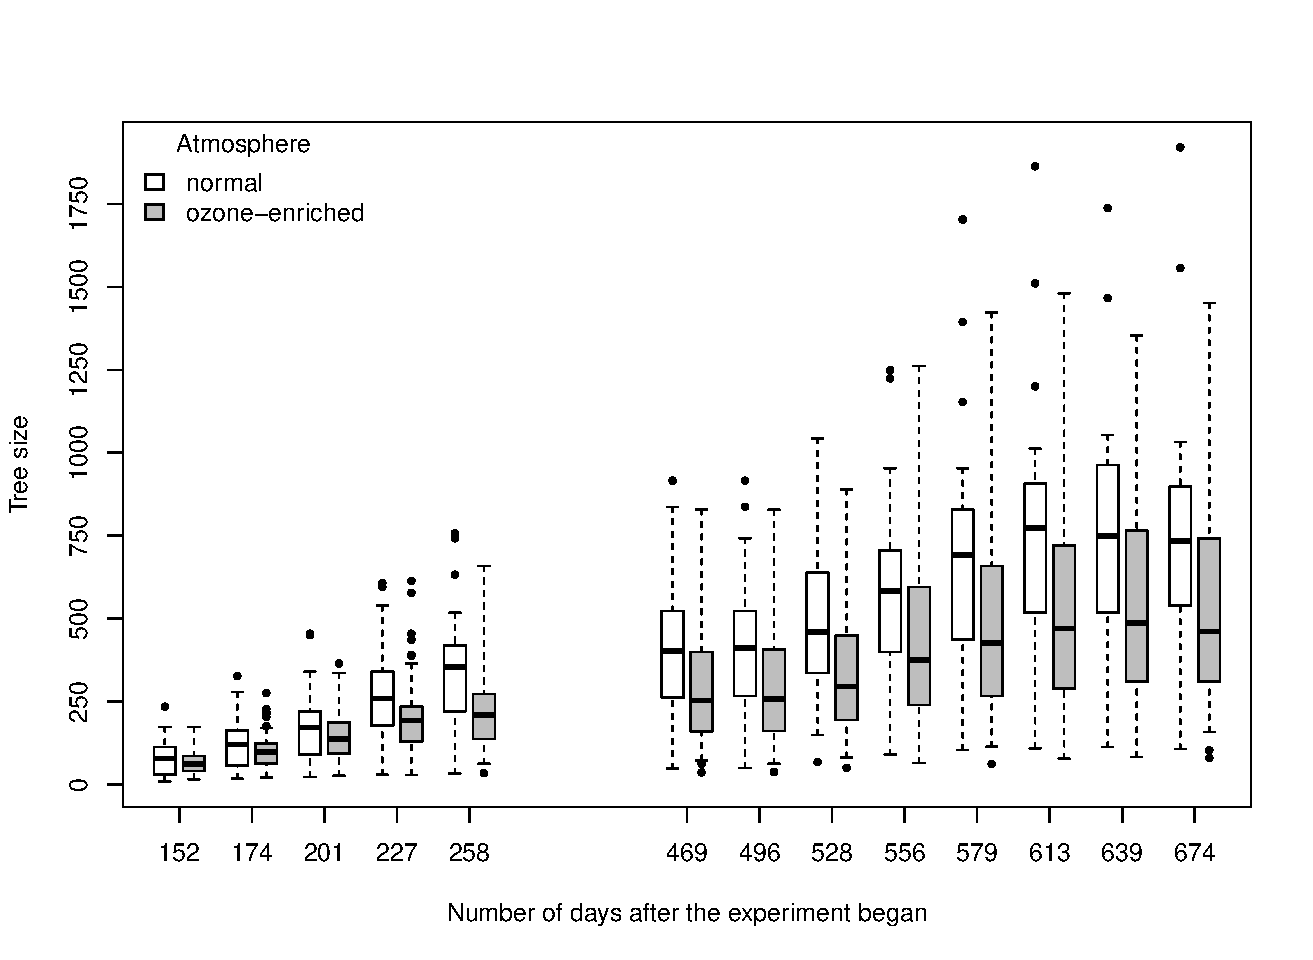
\includegraphics[width=\textwidth]{spruces}
\caption{Growth patterns of trees under normal and ozone-enriched atmospheres.}
\label{spruces0}
\end{figure}

%\begin{figure}[h!]
%\centering
%\psfrag{+}[][][0.4]{$\bullet$}
%\psfrag{e}[][][0.8]{Tree size}
%\psfrag{d}[][][0.8]{\hspace{-1cm}Number of days after the experiment began}
%\psfrag{c}[][][0.8]{\hspace{1cm}Atmosphere}
%\psfrag{a}[][][0.7]{\hspace{1cm}normal}
%\psfrag{b}[][][0.7]{\hspace{2.3cm}ozone-enriched}
%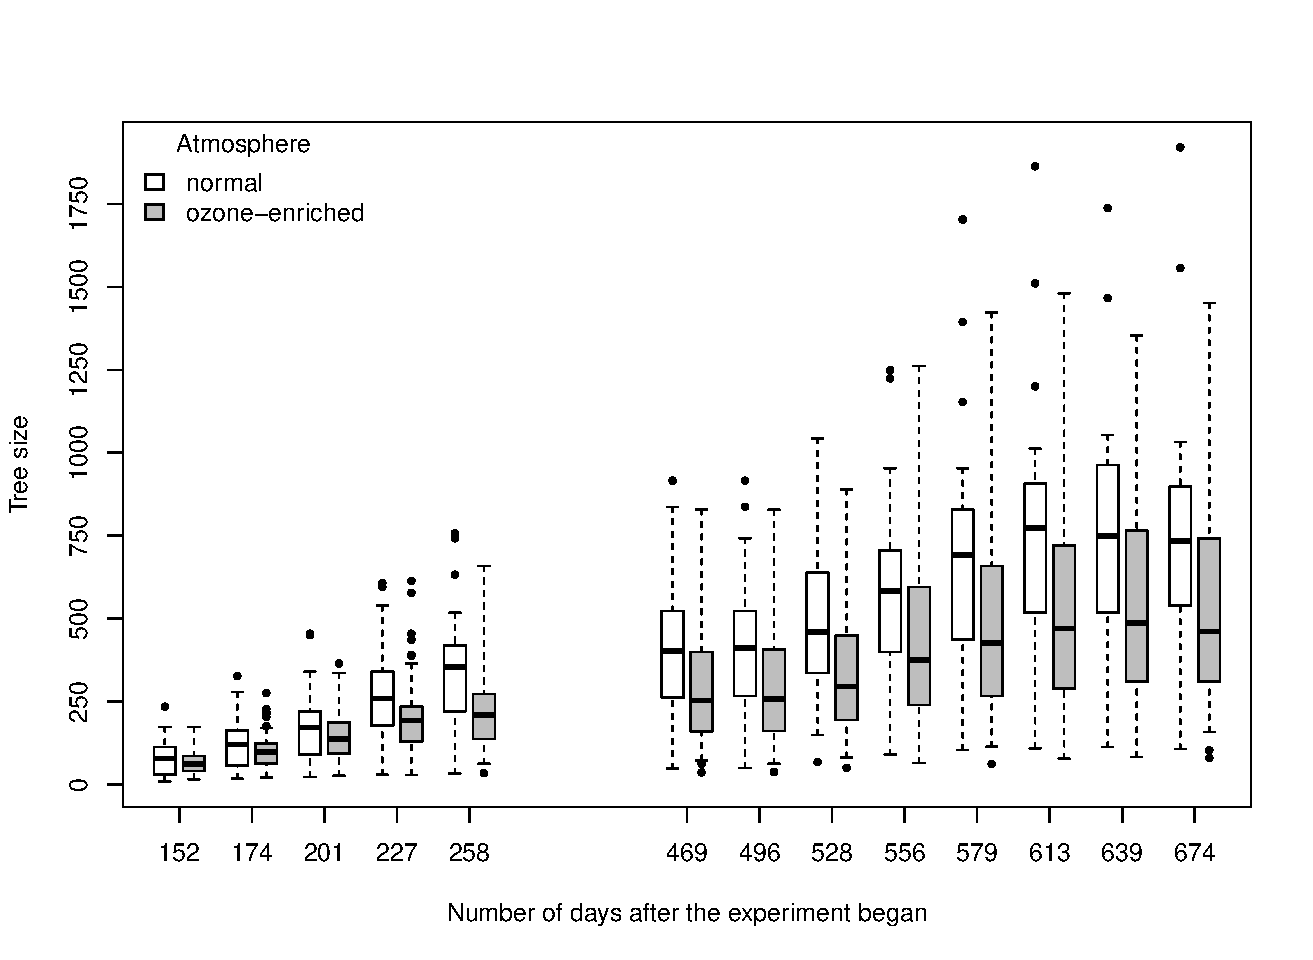
\includegraphics[width=\textwidth]{spruces}
%\caption{Growth patterns of trees under normal and ozone-enriched atmospheres.}
%\label{spruces0}
%\end{figure}

Plots (not shown here) of the deviance-type residuals versus the fitted values for two GEE with logarithmic link, working correlation matrix specified to be the identity matrix, and variance functions ${\rm V}(\mu) = \mu$ and ${\rm V}(\mu) = \mu^3$, reveal megaphone shaped and inverted megaphone shaped patterns, respectively, indicating thus how inappropriate such variance functions are for describing the heteroscedasticity present in the data. On the other hand, the same plot but using the variance function ${\rm V}(\mu) = \mu^2$ (Figure~\ref{spruces}(a)) does not reveal any trend, indicating that the data could be suitably analyzed under the assumption of a constant coefficient of variation. So, several GEE with the variance function ${\rm V}(\mu) = \mu^2$, logarithmic link, and different structures for the working correlation matrix are fitted to the data. Then, the selection criteria available in {\tt glmtoolbox} are used to choose the more suitable structure for the correlation matrix.

\begin{example}
> data(spruces)
> m1 <- glmgee(size ~ poly(days,4) + treat, id=tree, family=Gamma(log), data=spruces)
> m2 <- update(m1, corstr="Exchangeable")
> m3 <- update(m1, corstr="AR-M-dependent(1)")
> m4 <- update(m1, corstr="AR-M-dependent(2)")
> m5 <- update(m1, corstr="AR-M-dependent(3)")

> a <- CIC(m1, m2, m3, m4, m5, verbose=FALSE)
> b <- QIC(m1, m2, m3, m4, m5, verbose=FALSE)
> c <- GHYC(m1, m2, m3, m4, m5, verbose=FALSE)
> d <- RJC(m1, m2, m3, m4, m5, verbose=FALSE)
> e <- AGPC(m1, m2, m3, m4, m5, verbose=FALSE)
> f <- SGPC(m1, m2, m3, m4, m5, verbose=FALSE)
> cbind(a,QIC=b[,"QIC"],GHYC=c[,"GHYC"],RJC=d[,"RJC"],AGPC=e[,"AGPC"],SGPC=f[,"SGPC"])

  Object       Correlation   CIC   QIC   GHYC    RJC  AGPC  SGPC
1     m1      Independence 23.43 42068 116.42 41.303 13539 13554
2     m2      Exchangeable 23.43 42068  40.96  7.639 11689 11706
3     m3 AR-M-dependent(1) 23.66 42086  11.26  0.129 10941 10957
4     m4 AR-M-dependent(2) 23.56 42158  13.72  0.489 10981 11000
5     m5 AR-M-dependent(3) 23.56 42201  12.45  0.914 10994 11016
\end{example}

Most of the selection criteria (that is, Gosho-Hamada-Yoshimura’s criterion, Rotnitzky-Jewell’s criterion, Akaike-type penalized Gaussian pseudo-likelihood criterion, and Schwarz-type penalized Gaussian pseudo-likelihood criterion) suggest the first-order autoregressive (AR-1) and Independence as the more and less adequate structures for the correlation matrix, respectively. GEE with the AR-1 structure for the correlation matrix is summarized as follows:

\begin{example}
> summary(m3)
Sample size
   Number of observations:  1027
       Number of clusters:  79 
             Cluster size:  13 
*********************************************************************
Model
        Variance function:  Gamma
            Link function:  log
    Correlation structure:  AR-M-dependent(1)
*********************************************************************
Coefficients
                     Estimate Std.Error   z-value Pr(>|z|)
(Intercept)           5.90378   0.10486  56.30321  < 2e-16
poly(days, 4)1       19.20015   0.51848  37.03159  < 2e-16
poly(days, 4)2       -2.85755   0.20585 -13.88147  < 2e-16
poly(days, 4)3        5.41639   0.18246  29.68549  < 2e-16
poly(days, 4)4       -3.57407   0.12478 -28.64405  < 2e-16
treatozone-enriched  -0.25861   0.12835  -2.01486 0.043919
                                                          
Dispersion            0.32866                             
*********************************************************************
Working correlation
     [1]  [2]  [3]  [4]  [5]  [6]  [7]  [8]  [9]  [10] [11] [12] [13] 
[1]  1.00 0.97 0.93 0.90 0.87 0.84 0.81 0.78 0.76 0.73 0.70 0.68 0.66
[2]  0.97 1.00 0.97 0.93 0.90 0.87 0.84 0.81 0.78 0.76 0.73 0.70 0.68
[3]  0.93 0.97 1.00 0.97 0.93 0.90 0.87 0.84 0.81 0.78 0.76 0.73 0.70
[4]  0.90 0.93 0.97 1.00 0.97 0.93 0.90 0.87 0.84 0.81 0.78 0.76 0.73
[5]  0.87 0.90 0.93 0.97 1.00 0.97 0.93 0.90 0.87 0.84 0.81 0.78 0.76
[6]  0.84 0.87 0.90 0.93 0.97 1.00 0.97 0.93 0.90 0.87 0.84 0.81 0.78
[7]  0.81 0.84 0.87 0.90 0.93 0.97 1.00 0.97 0.93 0.90 0.87 0.84 0.81
[8]  0.78 0.81 0.84 0.87 0.90 0.93 0.97 1.00 0.97 0.93 0.90 0.87 0.84
[9]  0.76 0.78 0.81 0.84 0.87 0.90 0.93 0.97 1.00 0.97 0.93 0.90 0.87
[10] 0.73 0.76 0.78 0.81 0.84 0.87 0.90 0.93 0.97 1.00 0.97 0.93 0.90
[11] 0.70 0.73 0.76 0.78 0.81 0.84 0.87 0.90 0.93 0.97 1.00 0.97 0.93
[12] 0.68 0.70 0.73 0.76 0.78 0.81 0.84 0.87 0.90 0.93 0.97 1.00 0.97
[13] 0.66 0.68 0.70 0.73 0.76 0.78 0.81 0.84 0.87 0.90 0.93 0.97 1.00
\end{example}

The Wald test and the generalized score test suggest that there is no interaction between time and the type of atmosphere. This is because, as shown below, the $p$-values associated with that effect are ``large''. 

\begin{example}
> m3a <- update(m3, . ~ . + poly(days,4):treat)
> anova(m3a, test="wald")
Wald test 

Model 1 :  size ~ 1 
Model 2 :  size ~ poly(days, 4) 
Model 3 :  size ~ poly(days, 4) + treat 
Model 4 :  size ~ poly(days, 4) + treat + poly(days, 4):treat 

           Chi    df   Pr(>Chi)    
1 vs 2 1931.9813   4    < 2e-16 ***
2 vs 3    4.0597   1    0.04392 *  
3 vs 4    3.6641   4    0.45336 

> anova(m3a, test="score")
Generalized score test 

Model 1 :  size ~ 1 
Model 2 :  size ~ poly(days, 4) 
Model 3 :  size ~ poly(days, 4) + treat 
Model 4 :  size ~ poly(days, 4) + treat + poly(days, 4):treat 

         Chi    df   Pr(>Chi)    
1 vs 2 61.3028   4  1.544e-12 ***
2 vs 3  3.3687   1    0.06645 .  
3 vs 4  3.4665   4    0.48300   
\end{example}

\subsubsection{Variance estimation}
Next, the estimates of ${\rm Var}(\hat{\beta}_0),{\rm Var}(\hat{\beta}_1),\ldots,{\rm Var}(\hat{\beta}_5)$ are obtained using four different estimators.
\begin{example}
> cbind(model=diag(vcov(m3, type="model")), 
+       robust=diag(vcov(m3, type="robust")), 
+       bias.corrected=diag(vcov(m3, type="bias-corrected")),
+       jackknife=diag(vcov(m3, type="jackknife")))
                     model robust bias.corrected jackknife
(Intercept)         0.0110 0.0110         0.0119    0.0119
poly(days, 4)1      0.2564 0.2688         0.2758    0.2758
poly(days, 4)2      0.0922 0.0424         0.0435    0.0435
poly(days, 4)3      0.0352 0.0333         0.0342    0.0342
poly(days, 4)4      0.0283 0.0156         0.0160    0.0160
treatozone-enriched 0.0159 0.0165         0.0176    0.0176
\end{example}

\subsubsection{Parameter interpretation}
Across time, the expected size of the trees that grew under the ozone-enriched atmosphere is approximately $22.79\% = 100\times[1-\exp(\hat{\beta}^{\rm treat})]$ lower than that of the trees that grew under the normal atmosphere, where $\beta^{\rm treat}$ represents the parameter associated with the dummy variable indicating the type of atmosphere under which the trees grew. According to the Wald test, the hypothesis ${\rm H}_0: {\beta}^{\rm treat} \geq 0$ versus ${\rm H}_1: {\beta}^{\rm treat} < 0$ is rejected at the approximate level of $5\%$, indicating thus that the ozone-enriched atmosphere suppresses tree growth. 

\subsubsection{Variable selection}
As an illustration, the procedure of variable selection is applied using the strategy ``hybrid forward stepwise'' with the $p$-value of the generalized score test as the comparison criterion, and where the thresholds for add and drop effects are set at $10\%$ and $5\%$, respectively. In addition, the simplest and most complex models are specified to be {\tt 1} and {\tt 1+poly(days,4)+treat+poly(days,4):treat}, respectively. As shown below, the best linear predictor according to the chosen strategy incorporates both time and atmosphere, but not the interaction between them. The same results are obtained when the strategy of variable selection is changed as follows: $(i)$ the generalized score test is replaced by the Wald test; $(ii)$ and the ``hybrid forward stepwise'' procedure is replaced by the ``hybrid backward stepwise''.
 
\begin{example}
stepCriterion(m3, direction="forward", criterion="p-value", test="score",
+             scope=list(lower=~1, upper=~poly(days,4)*treat), levels=c(0.10,0.05))

    Variance function:  Gamma
        Link function:  log 
Correlation structure:  AR-M-dependent(1) 
  Comparison criteria:  P(Chisq>)(*)

Initial model:
~ 1 

Step 0 :
                       df   QIC  QICu  AGPC  SGPC P(Chisq>)(*)
+ poly(days, 4)         4 39944 39928 10927 10941    1.544e-12
+ treat                 1 19534 19517 12353 12360      0.03618
<none>                    18998 18989 12362 12367             

Step 1 : + poly(days, 4) 

                       df   QIC  QICu  AGPC  SGPC P(Chisq>)(*)
+ treat                 1 42086 42051 10941 10957      0.06645
<none>                    39944 39928 10927 10941             

Step 2 : + treat 

                       df   QIC  QICu  AGPC  SGPC P(Chisq>)(*)
+ poly(days, 4):treat   4 41815 41787 10954 10980        0.483
<none>                    42086 42051 10941 10957             

Final model:
~ poly(days, 4) + treat 
****************************************************************************
(*) p-values of the generalized score test
 Effects are added when their p-values are lower than 0.1
 Effects are excluded when their p-values are higher than 0.05
\end{example}

\begin{figure}[h!]
\centering
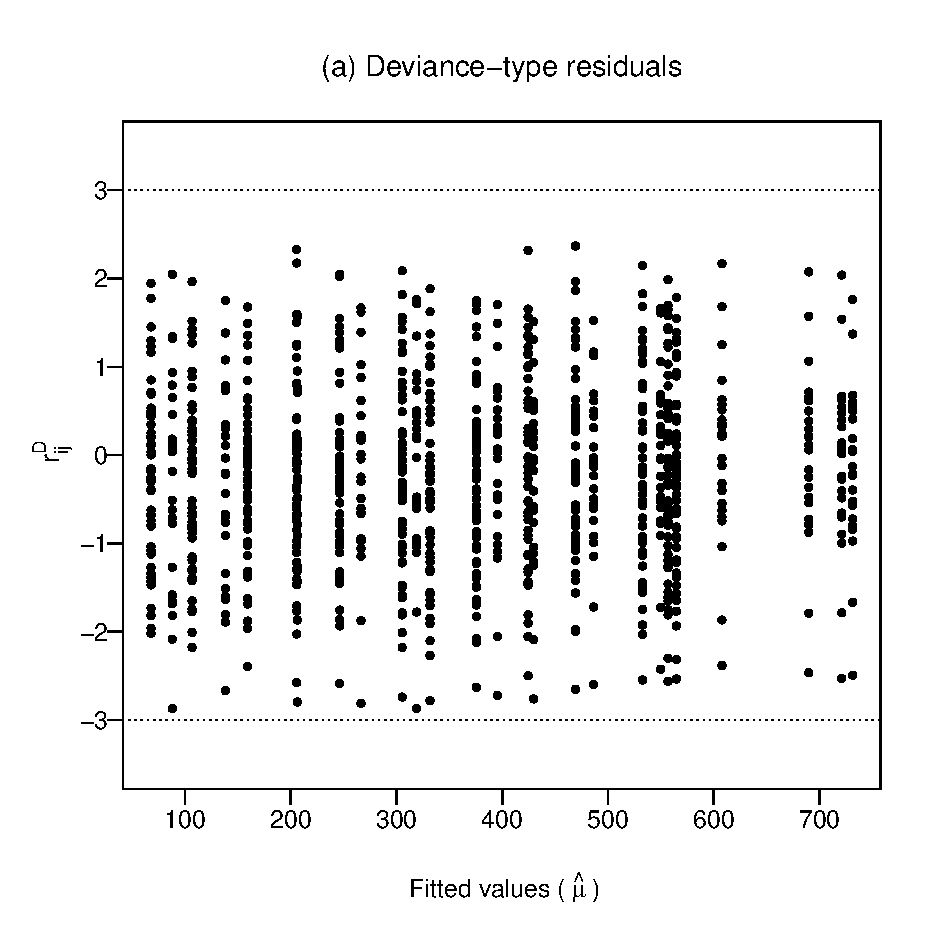
\includegraphics[width=6.75cm]{spruces3a}
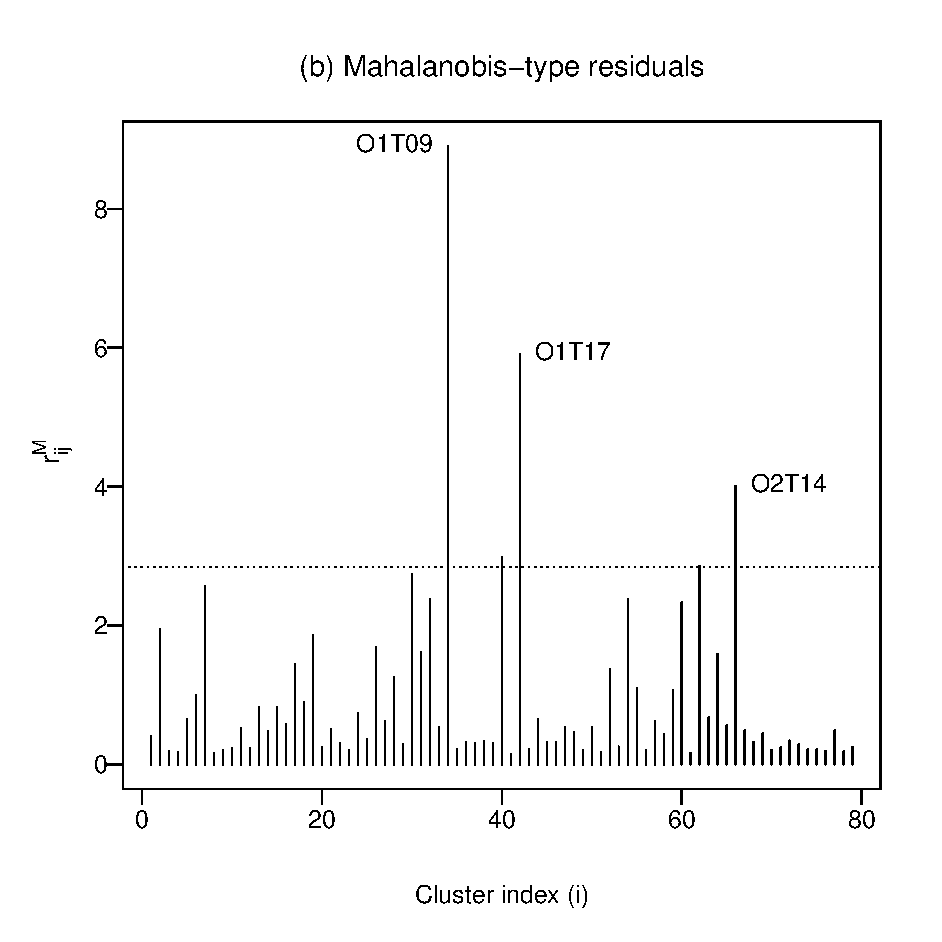
\includegraphics[width=6.75cm]{spruces3b}\\
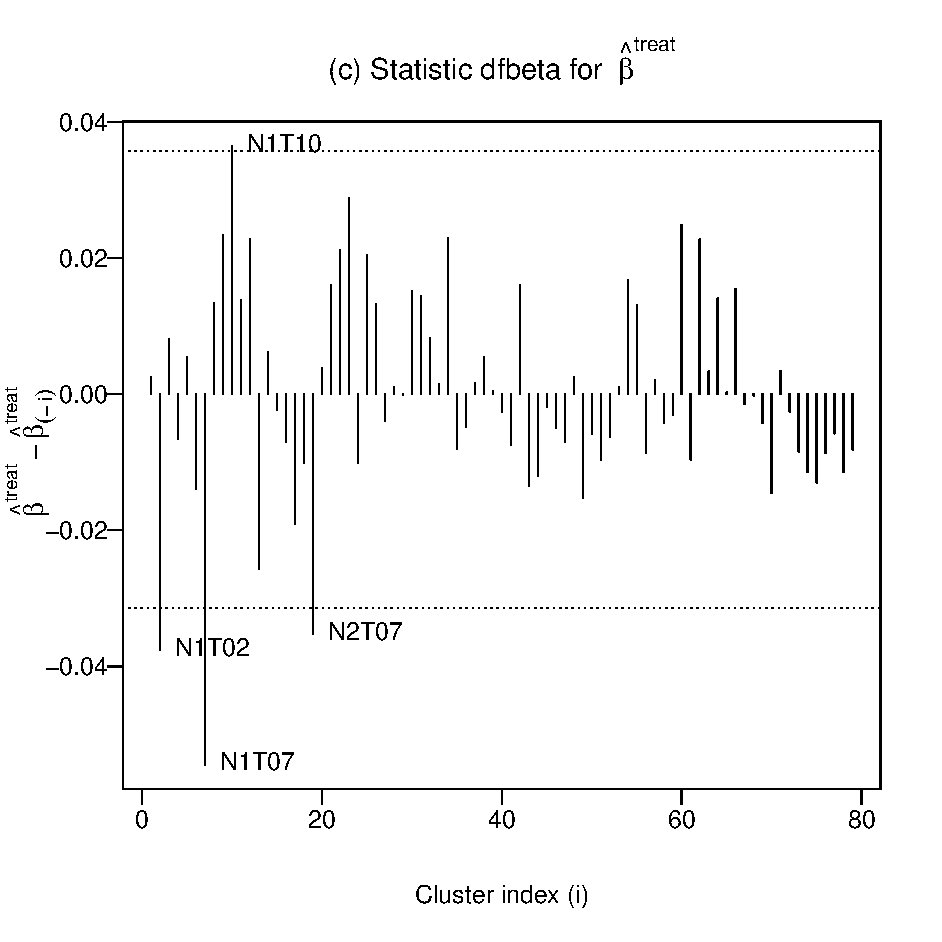
\includegraphics[width=6.75cm]{spruces3c}
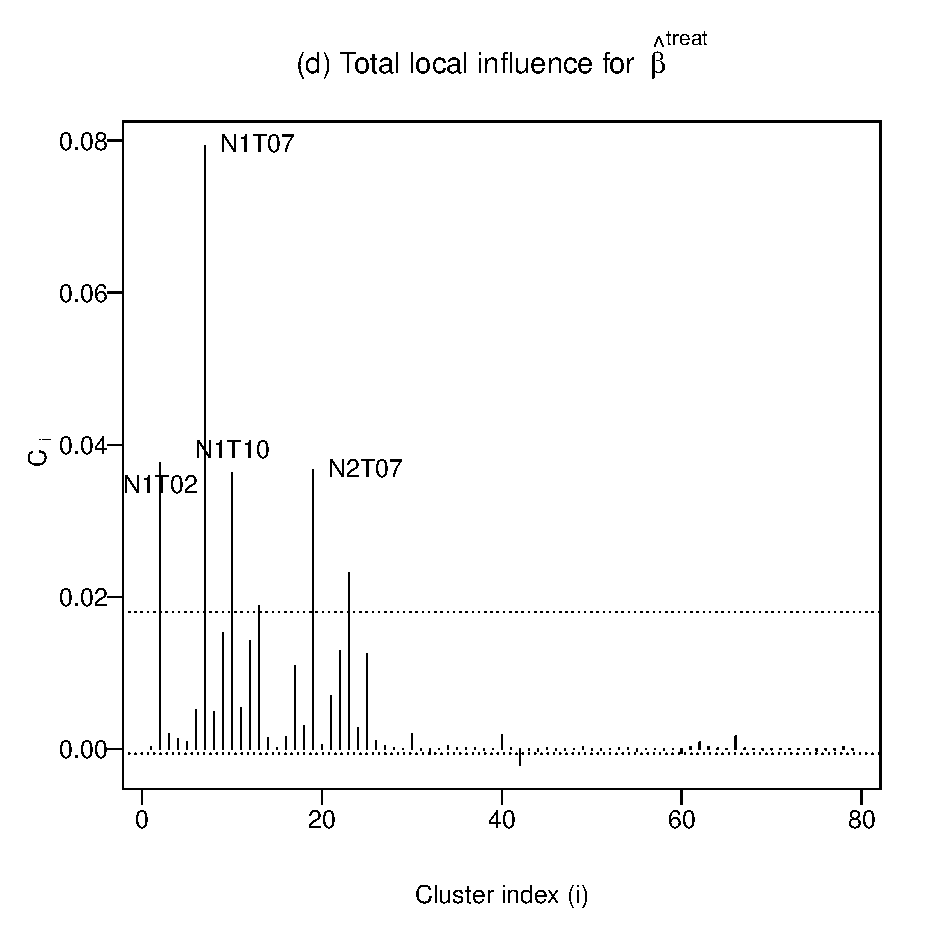
\includegraphics[width=6.75cm]{spruces3d}
\caption{Some diagnostic plots for the GEE with correlation structure AR-1 fitted to the data on growth
patterns of trees.}
\label{spruces}
\end{figure}

%\begin{figure}[h!]
%\centering
%\psfrag{+}[][][0.4]{$\bullet$}
%\psfrag{b}[][][0.8][-90]{$r^{D}_{ij}$}
%\psfrag{i}[][][0.8][-90]{$C_{ii}$}
%\psfrag{g}[][][0.8][0]{$\hat{\beta}^{\rm treat}-\hat{\beta}^{\rm treat}_{_{\!(-i)}}$}
%\psfrag{e}[][][0.8][-90]{$r^{M}_{i}$}
%\psfrag{a}[][][0.8]{\hspace{-0.3cm}Fitted values ($\hat{\mu}$)}
%\psfrag{d}[][][0.8]{\hspace{-0.3cm}Cluster index ($i$)}
%\psfrag{c}[][][0.8]{\hspace{-1cm}(a) Deviance-type residuals}
%\psfrag{f}[][][0.8]{\hspace{-1cm}(b) Mahalanobis-type residuals}
%\psfrag{h}[][][0.8]{\hspace{-0.8cm}(c) Statistic dfbeta for $\hat{\beta}^{\rm treat}$}
%\psfrag{j}[][][0.8]{\hspace{-0.8cm}(d) Total local influence for $\hat{\beta}^{\rm treat}$}
%\includegraphics[width=\textwidth]{spruces2}\\
%\includegraphics[width=\textwidth]{spruces3}
%\caption{Some diagnostic plots for the GEE with correlation structure AR-1 fitted to the data on growth
%patterns of trees.}
%\label{spruces}
%end{figure}

\subsubsection{Residual analysis}
\begin{example}
> residuals(m3, type="deviance", plot.it=TRUE, pch=16)
> residuals(m3, type="mahalanobis", plot.it=TRUE, identify=3)
\end{example}

According to the Mahalanobis-type residuals (Figure~\ref{spruces}(b)) the trees for which the model has the lowest goodness-of-fit are those identified as O1T09, O1T17 and O2T14. Although those trees grew under an ozone-enriched atmosphere, which seems to be associated with expected sizes lower than those of the trees which grew under the normal atmosphere, their observed sizes across the time are even greater than those observed for $70\%$ of the trees which grew under a normal atmosphere.

\subsubsection{Global influence}
\begin{example}
> dfbeta(m3, method="full", coefs="treat", identify=4)
\end{example}

According to the statistic Dfbeta at the cluster-level for $\hat{\beta}^{\rm treat}$ (Figure~\ref{spruces}(c)), the trees known as N1T02, N1T07 and N2T07 are those providing the greatest evidence which supports the negative effect of the ozone-enriched atmosphere on the growth pattern of the trees, as their exclusion from the dataset leads the estimate of $\beta^{\rm treat}$ closer to zero. Those trees grew under a normal atmosphere, and their sizes across time are higher than those observed for $90\%$ of the trees growing under such an atmosphere. On the other hand, the tree identified as N1T10 is that providing the greatest evidence against the negative effect of the ozone-enriched atmosphere on the growth pattern of the trees, because its exclusion from the dataset decreases the estimate of $\beta^{\rm treat}$. The tree identified as N1T10 grew under a normal atmosphere, however, its size across time is lower than that observed for $90\%$ of the trees growing under the ozone-enriched atmosphere.

\subsubsection{Local influence}
\begin{example}
> localInfluence(m3, type="total", perturbation="cw-clusters", coefs="treat", 
+                plot.it=TRUE, identify=4)
\end{example}

The plot of the total local influence under the case weight perturbation scheme at the cluster-level for $\hat{\beta}^{\rm treat}$ (Figure~\ref{spruces}(d)) highlights the trees identified as N1T07, N1T02, N2T07 and N1T10 as suspected to be influential on the estimate of $\beta^{\rm treat}$, which confirms the results of the global influence analysis above.

\subsection{Comparison with other GEE solvers}
The parameter estimates and the associated standard errors provided by the function {\tt glmgee()} are compared with those generated by the GEE solvers available in the packages {\tt gee}, {\tt geepack} and {\tt geeM}. The results are presented in Table~\ref{GeesS}. The values provided by the other GEE solvers are very similar to those generated by the function {\tt glmgee()}.

\begin{table}[!ht]
{\small
\begin{center}
\begin{tabular}{ccccc} 
 \hline                                                                       
                    & {\tt glmtoolbox}& {\tt geepack} & {\tt gee}     & {\tt geeM} \\\hline                                                               
(Intercept)         &  \hfill  5.904(0.105) &  \hfill 5.903(0.105) & \hfill  5.904(0.105) & \hfill  5.904(0.105)\\                                              poly(days, 4)1      &  \hfill 19.200(0.518) & \hfill 19.186(0.519) & \hfill 19.201(0.518) & \hfill 19.200(0.518)\\
poly(days, 4)2      &  \hfill -2.858(0.206) & \hfill -2.860(0.206) & \hfill -2.857(0.206) & \hfill -2.858(0.206)\\
poly(days, 4)3      &  \hfill  5.416(0.182) & \hfill 5.414(0.182)  & \hfill  5.417(0.182) & \hfill  5.416(0.182)\\
poly(days, 4)4      &  \hfill -3.574(0.125) & \hfill -3.572(0.125) & \hfill -3.574(0.125) & \hfill -3.574(0.125)\\
treatozone-enriched &  \hfill -0.259(0.128) & \hfill -0.257(0.128) & \hfill -0.259(0.128) & \hfill -0.259(0.128)\\
$\rho$              &               0.97    &       0.97           &        0.97          & 0.97\\\hline
\end{tabular}
\end{center}
\caption{Parameter estimates (standard errors) of the GEE model with correlation structure AR-1 fitted to the data on growth
patterns of trees.}
\label{GeesS}}
\end{table}
                                                                                                                                                                 
\subsection{Treatment of severe postnatal depression}
The dataset of this example, available in the object {\tt depression} of {\tt glmtoolbox} and composed of columns named {\tt subj}, {\tt group}, {\tt visit}, {\tt dep} and {\tt depressd} (see Table~\ref{td}), arose from a double-blind placebo-controlled study on the efficacy of oestrogen given transdermally for treatment of severe postnatal depression \citep{GKES96}. A total of 61 women with severe depression (identified in the dataset by the column {\tt subj}), which began within 3 months of childbirth and persisted for up to 18 months postnatal, were randomly assigned to either a control group ({\tt group=``placebo''}) of size 27, which were treated with a placebo patch, or an active treatment group ({\tt group=``oestrogen''}) of size 34, which were treated with an oestrogen patch. Prior to therapy, all women were assessed by self-ratings of depressive symptoms on the Edinburgh Postnatal Depression Scale (EPDS), where higher scores are indicative of higher levels of depression. A monthly EPDS (dep) was collected for six months once treatment began ({\tt visit}). The binary response ({\tt depressd}) was 1 to indicate severe depression when the EDPS value was greater than or equal to 11, and 0 in other cases. There are missing values in the data, because for some women, just two measurements of the response variable are available. However, those missing values are positioned at the last time positions, so, there are no intermixed missing values, and the argument {\tt waves} of the function {\tt glmgee()} is not needed. 

\begin{table}[!ht]
{\small
\begin{center}
\begin{tabular}{lll} 
 \hline
Column &  Role   &  Description\\ \hline
{\tt subj}  & Cluster/subject identifier & Identifier of the woman\\
{\tt group} & Explanatory variable & Treatment: ``placebo'' or ``oestrogen''\\
{\tt visit} & Explanatory variable & Number of months after the treatment began\\
{\tt depressd} & Response variable& 1 if ${\rm EDPS}\geq 11$ and 0 otherwise\\ 
 \hline
\end{tabular}
\end{center}
\caption{Columns in the object {\tt depression} of the package {\tt glmtoolbox}.}
\label{td}}
\end{table}

A plot of the data (Figure~\ref{depression0}) suggests that oestrogen patches are an effective treatment for postnatal severe depression, as across time, the proportion of women with severe depression is lower in the group treated with oestrogen patches than in the group treated with placebo patches. The plot also indicates that the (logit of the) proportion of women with severe depression decreases linearly as a function of the time since the therapy began, but the rate of decreasing seems to be independent of the type of patch (placebo or oestrogen), which suggests that the data could be analyzed by using a GEE with the logit link function and a linear predictor including the effects of time and type of patch, but without the interaction between them.

\begin{figure}[h!]
\centering
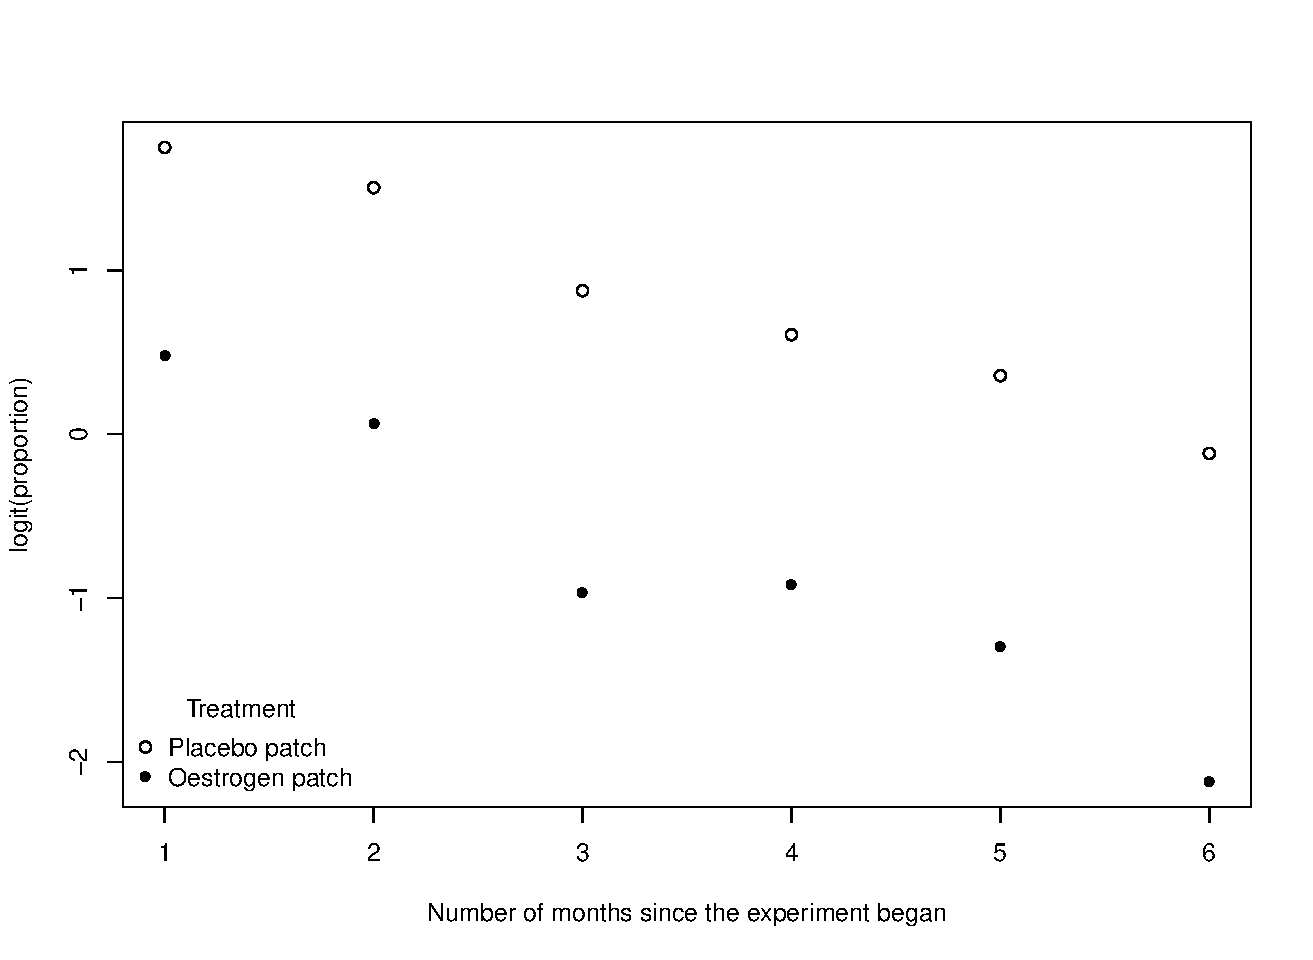
\includegraphics[width=\textwidth]{depression1}
\caption{Evolution of the (logit of the) proportion of women with severe depression.}
\label{depression0}
\end{figure}

%\begin{figure}[h!]
%\centering
%\psfrag{-2}[][][0.65]{$-2$}
%\psfrag{-1}[][][0.65]{$-1$}
%\psfrag{0}[][][0.65]{$0$}
%\psfrag{1}[][][0.65]{$1$}
%\psfrag{2}[][][0.65]{$2$}
%\psfrag{3}[][][0.65]{$3$}
%\psfrag{4}[][][0.65]{$4$}
%\psfrag{5}[][][0.65]{$5$}
%\psfrag{6}[][][0.65]{$6$}
%\psfrag{+}[][][0.65]{$\bullet$}
%\psfrag{-}[][][0.65]{$\circ$}
%\psfrag{a}[][][0.8]{\hspace{-1.3cm}Number of months since the experiment began}
%\psfrag{c}[][][0.65]{\hspace{2cm}Placebo patch}
%\psfrag{d}[][][0.65]{\hspace{2.3cm}Oestrogen patch}
%\psfrag{b}[][][0.8]{\hspace{-0.5cm}${\rm logit(proportion)}$}
%\psfrag{e}[][][0.7]{\hspace{1cm}Treatment}
%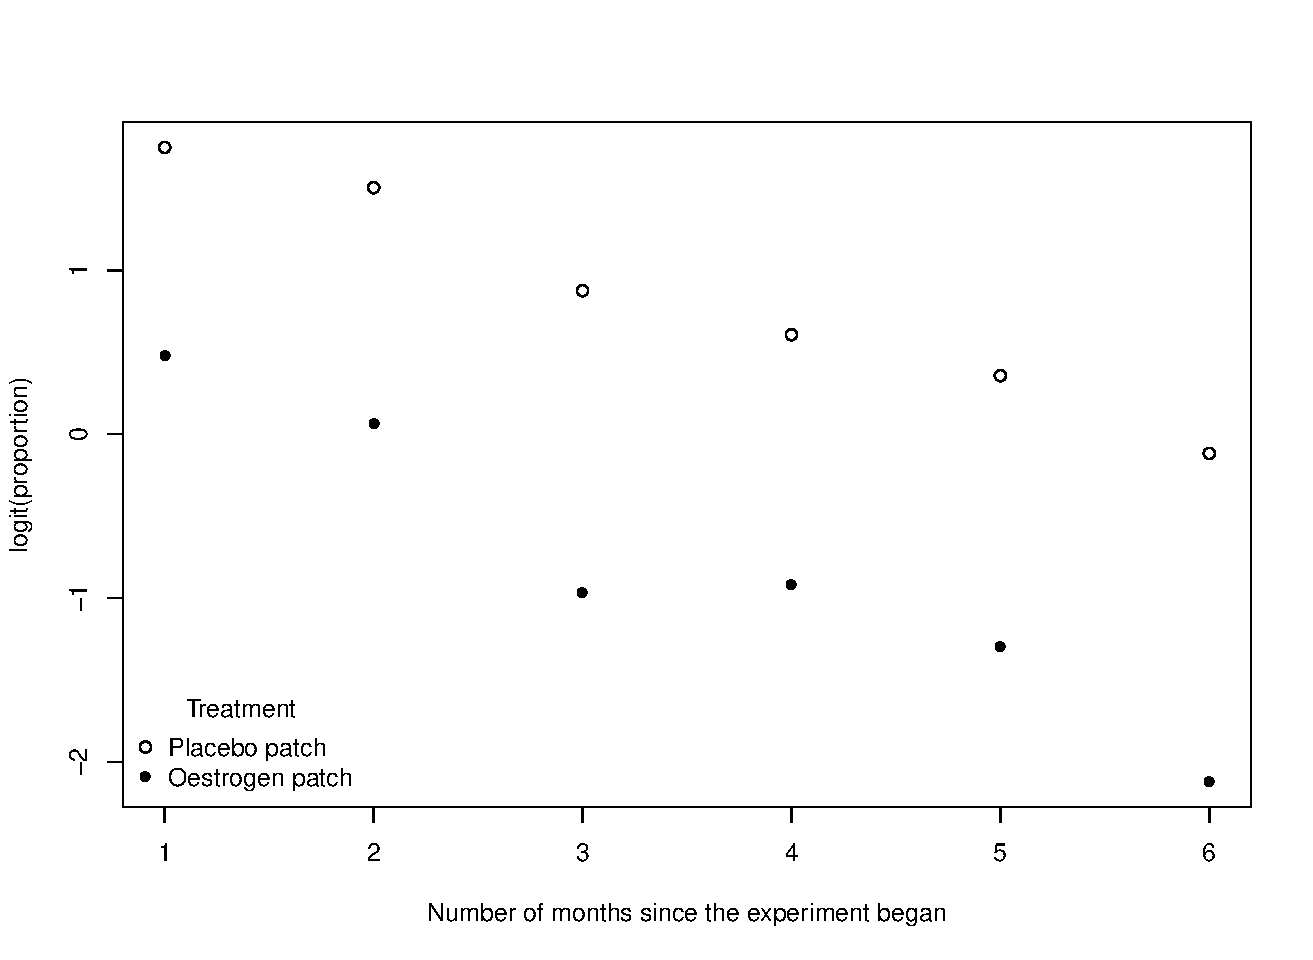
\includegraphics[width=\textwidth]{depression1}
%\caption{Evolution of the (logit of the) proportion of women with severe depression.}
%\label{depression0}
%\end{figure}

Several GEE with variance function ${\rm V}(\mu)=\mu(1-\mu)$, logit link function, and different structures for the working correlation matrix are fitted to the data. Then, some selection criteria available in {\tt glmtoolbox} are used to choose the more suitable structure for the correlation matrix.

\begin{example}
> data(depression)
> m1 <- glmgee(depressd ~ visit + group, id=subj, family=binomial(logit), data=depression)
> m2 <- update(m1, corstr="Exchangeable")
> m3 <- update(m1, corstr="AR-M-dependent(1)")
> m4 <- update(m1, corstr="AR-M-dependent(2)")
> m5 <- update(m1, corstr="AR-M-dependent(3)")

> a <- CIC(m1, m2, m3, m4, m5, verbose=FALSE)
> b <- QIC(m1, m2, m3, m4, m5, verbose=FALSE)
> c <- AGPC(m1, m2, m3, m4, m5, verbose=FALSE)
> d <- SGPC(m1, m2, m3, m4, m5, verbose=FALSE)
> cbind(a,QIC=b[,"QIC"],AGPC=c[,"AGPC"],SGPC=d[,"SGPC"])

  Object       Correlation  CIC    QIC     AGPC     SGPC
1     m1      Independence 7.708 383.555 304.2907 310.6233
2     m2      Exchangeable 8.048 377.815 247.9647 256.4082
3     m3 AR-M-dependent(1) 6.971 358.244 234.4696 242.9131
4     m4 AR-M-dependent(2) 7.031 363.784 234.9438 245.4982
5     m5 AR-M-dependent(3) 7.230 366.387 231.5530 244.2183
\end{example}

According to most of the selection criteria, the AR-1 structure is more suitable. Here is the summary of the GEE with that structure for the working correlation matrix:

\begin{example}
> summary(m3)
Sample size
   Number of observations:  356
       Number of clusters:  61 
                            Min  25%  50%  75%  Max
            Cluster sizes:    2    4    7    7    7
*********************************************************************
Model
        Variance function:  binomial
            Link function:  logit
    Correlation structure:  AR-M-dependent(1)
*********************************************************************
Coefficients
                Estimate Std.Error  z-value   Pr(>|z|)
(Intercept)     3.23604   0.51842  6.24218 4.3152e-10
visit          -0.62632   0.07477 -8.37681 < 2.22e-16
groupoestrogen -1.77723   0.54578 -3.25631  0.0011287
                                                    
Dispersion     1.02842                              
*********************************************************************
Working correlation
     [1]   [2]   [3]   [4]   [5]   [6]   [7] 
[1] 1.000 0.513 0.263 0.135 0.069 0.036 0.018
[2] 0.513 1.000 0.513 0.263 0.135 0.069 0.036
[3] 0.263 0.513 1.000 0.513 0.263 0.135 0.069
[4] 0.135 0.263 0.513 1.000 0.513 0.263 0.135
[5] 0.069 0.135 0.263 0.513 1.000 0.513 0.263
[6] 0.036 0.069 0.135 0.263 0.513 1.000 0.513
[7] 0.018 0.036 0.069 0.135 0.263 0.513 1.000
\end{example}

The Wald test and the generalized score test indicate that there is no interaction between time and the type of patch. As shown below, the $p$-values associated with that effect are ``large''.
\begin{example}
> m3a <- update(m3, . ~ . + visit:group)
> anova(m3a, test="wald")
Wald test 

Model 1 :  depressd ~ 1 
Model 2 :  depressd ~ visit 
Model 3 :  depressd ~ visit + group 
Model 4 :  depressd ~ visit + group + visit:group 

         Chi    df   Pr(>Chi)    
1 vs 2 88.1275   1  < 2.2e-16 ***
2 vs 3 10.6036   1   0.001129 ** 
3 vs 4  2.2104   1   0.137082

> anova(m3a, test="score")
Generalized score test 

Model 1 :  depressd ~ 1 
Model 2 :  depressd ~ visit 
Model 3 :  depressd ~ visit + group 
Model 4 :  depressd ~ visit + group + visit:group 

         Chi    df   Pr(>Chi)    
1 vs 2 39.9226   1  2.642e-10 ***
2 vs 3 10.9208   1  0.0009509 ***
3 vs 4  2.3977   1  0.1215150   
\end{example}

\subsubsection{Variance estimation}
Next, the estimates of ${\rm Var}(\hat{\beta}_0),{\rm Var}(\hat{\beta}_1),{\rm Var}(\hat{\beta}_2)$ are obtained using four different estimators.
\begin{example}
> cbind(model=diag(vcov(m3, type="model")), 
+       robust=diag(vcov(m3, type="robust")), 
+       bias.corrected=diag(vcov(m3, type="bias-corrected")),
+       jackknife=diag(vcov(m3, type="jackknife")))
                 model  robust bias.corrected jackknife
(Intercept)    0.26219 0.26875        0.29023   0.29023
visit          0.00844 0.00559        0.00583   0.00583
groupoestrogen 0.21114 0.29788        0.32441   0.32441
\end{example}

\subsubsection{Parameter interpretation}
Regardless of the type of patch (placebo or oestrogen), the probability of severe depression decreases across time. However, the odds of severe depression of women treated with oestrogen patches is approximately $83.09\% = 100\times[1-\exp(\hat{\beta}^{\rm group})]$ lower than that of women treated with placebo patches, where $\beta^{\rm group}$ represents the parameter associated with the dummy variable indicating the type of patch the women were treated with.

%\begin{figure}[h!]
%\centering
%\psfrag{b}[][][0.8][-90]{$r^{M}_{ij}$}
%\psfrag{a}[][][0.8]{\hspace{-0.3cm}Cluster index ($i$)}
%\psfrag{c}[][][0.8]{\hspace{-0.8cm}(a) Mahalanobis-type residuals}
%\psfrag{e}[][][0.8]{\hspace{-1cm}(b) Statistic dfbeta for $\hat{\beta}^{\rm group}$}
%\psfrag{d}[][][0.8][0]{$\hat{\beta}^{\rm group}-\hat{\beta}^{\rm group}_{_{\!(-i)}}$}
%\psfrag{f}[][][0.8][-90]{$C_{ii}$}
%\psfrag{h}[][][0.8]{\hspace{-0.6cm}Observation index}
%\psfrag{g}[][][0.8]{\hspace{-0.8cm}(c) Total local influence for $\hat{\beta}^{\rm group}$ at cluster-level}
%\psfrag{i}[][][0.8]{\hspace{-0.7cm}(d) Total local influence for $\hat{\beta}^{\rm group}$ at observation-level}
%\includegraphics[width=\textwidth]{depression2}\\
%\includegraphics[width=\textwidth]{depression3}
%\caption{Some diagnostic plots for the GEE with correlation structure AR-1 fitted to the data on severe
%postnatal depression.}
%\label{depression}
%\end{figure}

\begin{figure}[h!]
\centering
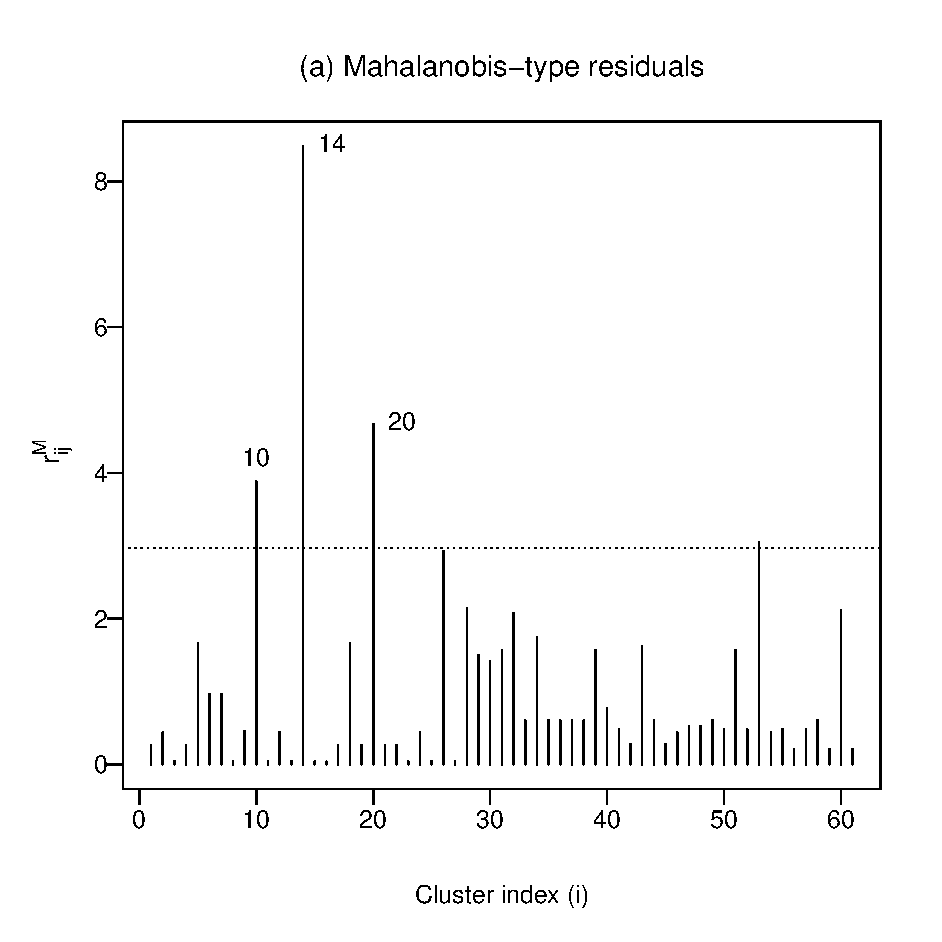
\includegraphics[width=6.75cm]{depression3a}
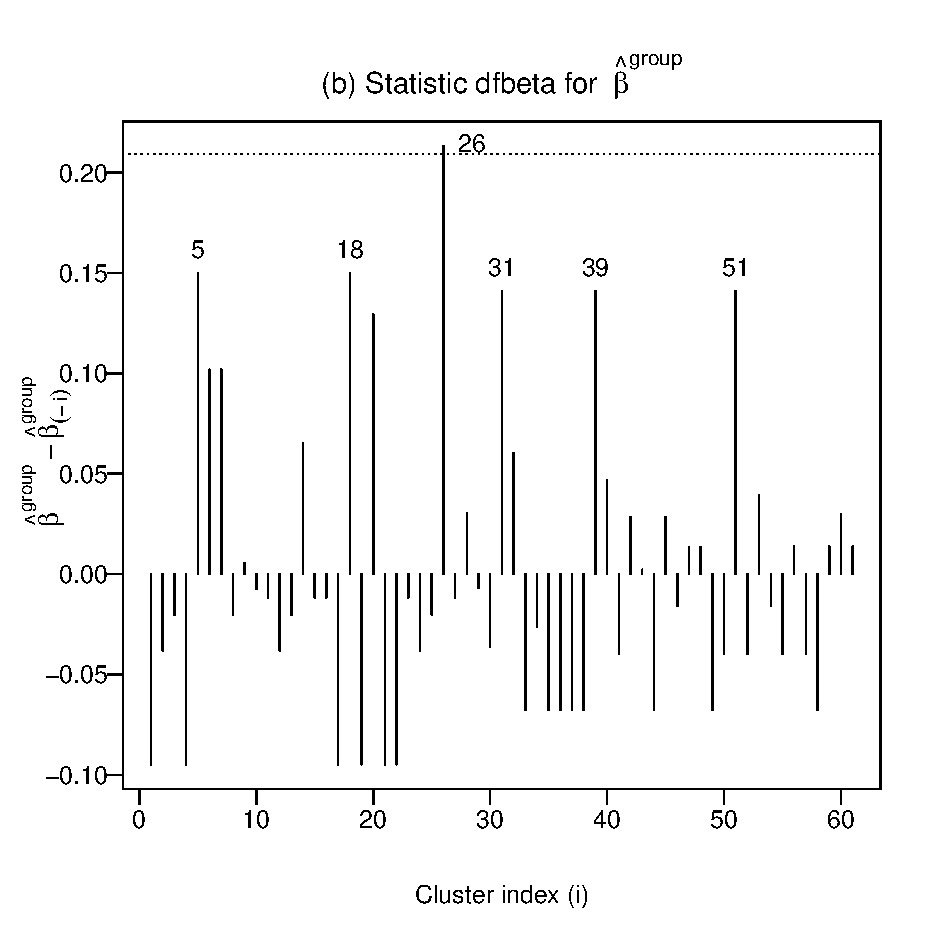
\includegraphics[width=6.75cm]{depression3b}\\
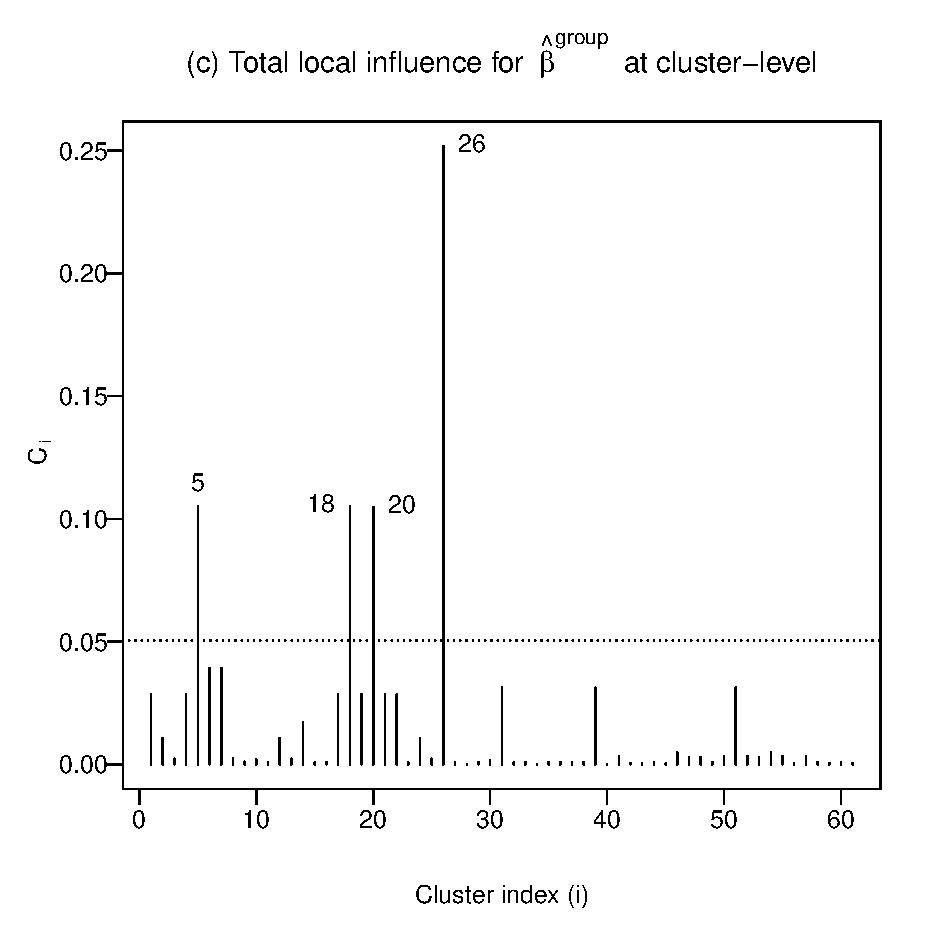
\includegraphics[width=6.75cm]{depression3c}
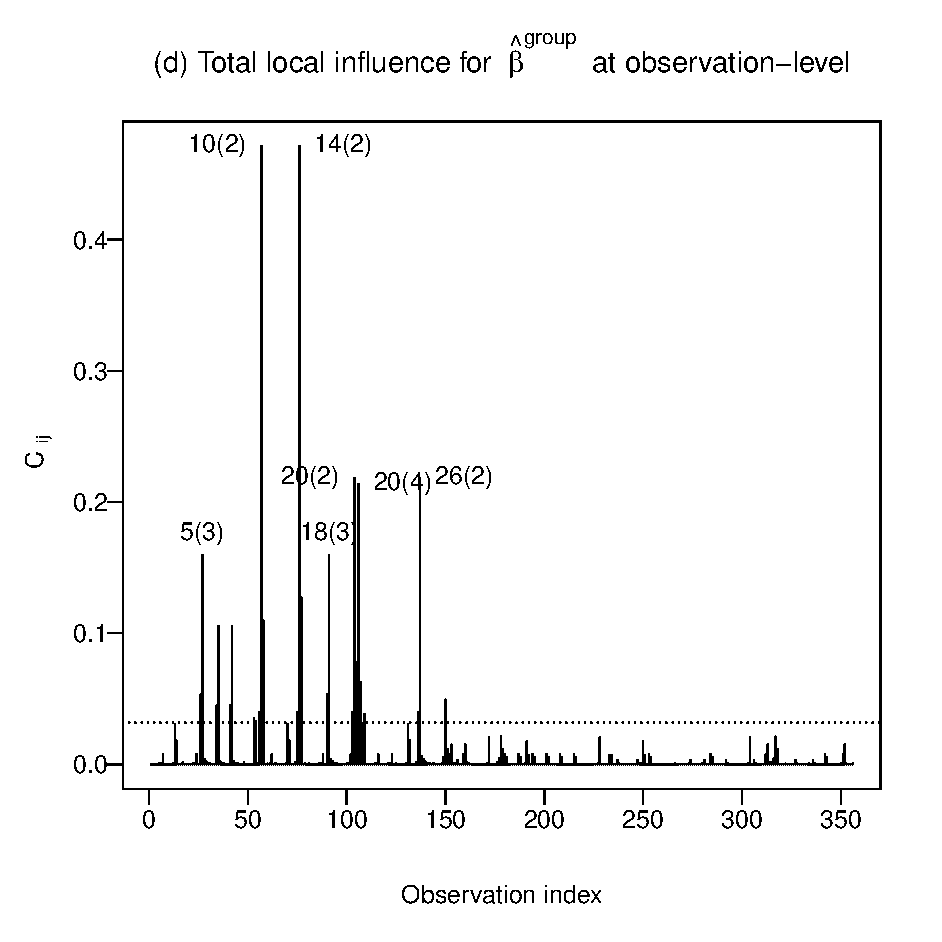
\includegraphics[width=6.75cm]{depression3d}
\caption{Some diagnostic plots for the GEE with correlation structure AR-1 fitted to the data on postnatal depression.}
\label{depression}
\end{figure}


\subsubsection{Variable selection}
As an illustration, the procedure of variable selection is applied using the strategy ``hybrid forward stepwise'' with the QIC as the comparison criterion. In addition, the simplest and most complex models are specified to be {\tt 1} and {\tt 1 + visit + group + visit*group}, respectively. According to this strategy, the ``best'' linear predictor consists of the effects of time and type of patch, but without the interaction between them. The same results are obtained in the following scenarios: $(i)$ the ``hybrid forward stepwise'' is replaced by the ``hybrid backward stepwise''; and $(ii)$ the comparison criterion based on the QIC is replaced by the AGPC.
\begin{example}
> stepCriterion(m3a, direction="forward", criterion="qic")

    Variance function:  binomial
        Link function:  logit 
Correlation structure:  AR-M-dependent(1) 
  Comparison criteria:  QIC

Initial model:
~ 1 

Step 0 :
               df    QIC   QICu   AGPC   SGPC P(Chisq>)(*)
+ visit         1 413.89 409.23 273.13 279.46    < 2.2e-16
+ group         1 443.77 440.13 366.77 373.10     0.000424
<none>            465.70 463.63 385.09 389.31             

Step 1 : + visit 

               df    QIC   QICu   AGPC   SGPC P(Chisq>)(*)
+ group         1 358.24 350.30 234.47 242.91     0.001129
<none>            413.89 409.23 273.13 279.46             

Step 2 : + group 

               df    QIC   QICu   AGPC   SGPC P(Chisq>)(*)
<none>            358.24 350.30 234.47 242.91             
+ group:visit   1 358.63 351.24 234.60 245.16       0.1371
- visit         1 443.77 440.13 366.77 373.10       <2e-16

Final model:
~ visit + group 
****************************************************************************
(*) p-values of the Wald test
\end{example}

\subsubsection{Residual analysis}
\begin{example}
> residuals(m3, type="mahalanobis", plot.it=TRUE, identify=3)
\end{example}

Mahalanobis-type residuals suggest that the women for whom the model has the lowest goodness-of-fit are those identified as 10, 14 and 20 (Figure~\ref{depression0}(a)). Those women were treated with placebo patches and just one month after therapy began their EDPS decreased until reaching values lower than 11. However, one or two months later their EDPS values increased to 11 or higher.

\subsubsection{Global influence}
\begin{example}
> dfbeta(m3, method="full", coefs="group", identify=6)
\end{example}

The plot of the dfbeta statistic for $\hat{\beta}^{\rm group}$ at the cluster-level (Figure~\ref{depression0}(b)) highlights the women identified as 5, 18, 26, 31, 39 and 51. The EDPS values of the women identified as 31, 39 and 51 remained higher or equal to 11 even after they were treated with oestrogen patches. Their exclusion from the dataset decreases the estimate of $\beta^{\rm group}$, that is, increases the evidence on the effectiveness of oestrogen patches for treatment of postnatal severe depression. On the other hand, the values on the EDPS of the women identified as 5, 18 and 26 remained lower than 11 since the first or second month since therapy began, although they were treated with placebo patches, so their exclusion from the dataset also increases the evidence on the effectiveness of the oestrogen patches for treatment of postnatal severe depression.

\subsubsection{Local influence}
\begin{example}
> localInfluence(m3, type="total", perturbation="cw-clusters", coefs="group", 
+                plot.it=TRUE, identify=4)
> localInfluence(m3, type="total", perturbation="cw-observations", coefs="group", 
+                plot.it=TRUE, identify=7)
\end{example}

According to the plot of the total local influence for $\hat{\beta}^{\rm group}$ under the case weight perturbation scheme at the cluster-level (Figure~\ref{depression0}(c)), the women identified as 5, 18, 20 and 26 are suspected to be influential on $\hat{\beta}^{\rm group}$. At least 4/7 of the EDPS measurements carried out on those women were smaller than 11, although they were supplied with placebo patches. The plot of the total local influence for $\hat{\beta}^{\rm group}$ under the case weight perturbation scheme at the observation-level (Figure~\ref{depression0}(d)) highlights mainly two kinds of observations: $(1)$ measurements of the EDPS in which, unlike the others measurements made on the same women, the values were lower than 11, although they were treated with placebo patches (second measurement performed on women identified as 10 and 14); $(2)$ measurements of the EDPS performed on women treated with placebo patches and in which, for the first time for those women since the treatment began, the reported value was lower than 11, thus indicating absent severe depression, which remains until the end of the observation period (second, third and fourth measurements performed on women identified as 26, 18 and 5, respectively).

\subsubsection{Comparison with other GEE solvers}
The parameter estimates and the associated standard errors provided by the function {\tt glmgee()} are compared with those calculated by the GEE solvers available in the packages {\tt gee}, {\tt geepack} and {\tt geeM}. The results are presented in Table~\ref{GeesD}. The values obtained with the other GEE solvers are very similar to those obtained with the function {\tt glmgee()}.

\begin{table}[!ht]
{\small
\begin{center}
\begin{tabular}{ccccc} 
 \hline                                                                       
                    & {\tt glmtoolbox}& {\tt geepack} & {\tt gee}  & {\tt geeM} \\\hline                                                               
(Intercept)         &  \hfill  3.236(0.518) & \hfill 3.276(0.531)  & \hfill  3.214(0.514) & \hfill  3.199(0.543)\\                                              visit               &  \hfill -0.626(0.075) & \hfill -0.630(0.077) & \hfill -0.624(0.074) & \hfill -0.633(0.077)\\
groupestrogen       &  \hfill -1.777(0.546) & \hfill -1.847(0.556) & \hfill -1.754(0.543) & \hfill -1.781(0.572)\\
$\rho$               &               0.51    &       0.48           &        0.47          & 0.51\\\hline
\end{tabular}
\end{center}
\caption{Parameter estimates (standard errors) of the GEE model with correlation structure AR-1 fitted to the data on severe
postnatal depression.}
\label{GeesD}}
\end{table}

\subsection{Growth patterns of two soybean genotypes}
This dataset, analyzed in \cite{DG95} and \cite{PB00} and available in the object {\tt Soybean} of the package {\tt nlme} \citep{PB22}, arose from an experiment aimed at comparing growth patterns of two genotypes of soybeans: Plant Introduction ({\tt Variety=``P''}), an experimental strain, and Forrest ({\tt Variety=``F''}), a commercial variety. The average leaf weight per plant ({\tt weight}), in grams, was measured at 14, 20, 27, 34, 41, 55, 69 and 84 days after planting ({\tt Time}) in each plot ({\tt Plot}). As an illustration, only plots planted in 1989 ({\tt Year=``1989''}) are analyzed here. Table ~\ref{Soy} describes the roles played in the analysis of the variables in the {\tt Soybean} dataset. The graph of the data (Figure \!~\ref{sg}) indicates that the location of the response (average leaf weight per plant) increases non-linearly over time. In addition, there is an approximately proportional relationship between the mean and the standard deviation, as the variance of the response variable (in the log scale) seems to be constant. As a result, the data may be analyzed assuming that the coefficient of variation is constant, that is, using a quadratic variance function. Moreover, the graph of the data also indicates that at each time point, the location of the response is larger for the experimental strain ({\tt Variety=``P''}) than for the commercial variety ({\tt Variety=``F''}) of soybean.

\begin{table}[!ht]
{\small
\begin{center}
\begin{tabular}{lll} 
 \hline
Column &  Role   &  Description\\ \hline
{\tt Plot}  & Cluster/subject identifier & Identifier of the plot\\
{\tt Variety} & Explanatory variable & Treatment: ``F'' (experimental) or ``P'' (commercial)\\
{\tt Year} & Explanatory variable & Year the plot was planted\\
{\tt Time} & Explanatory variable & Days after planting\\
{\tt weight} & Response variable& Average leaf weight per plant\\ 
 \hline
\end{tabular}
\end{center}
\caption{Columns in the object {\tt Soybean} of the package {\tt nlme}.}
\label{Soy}}
\end{table}

\begin{figure}[h!]
\centering
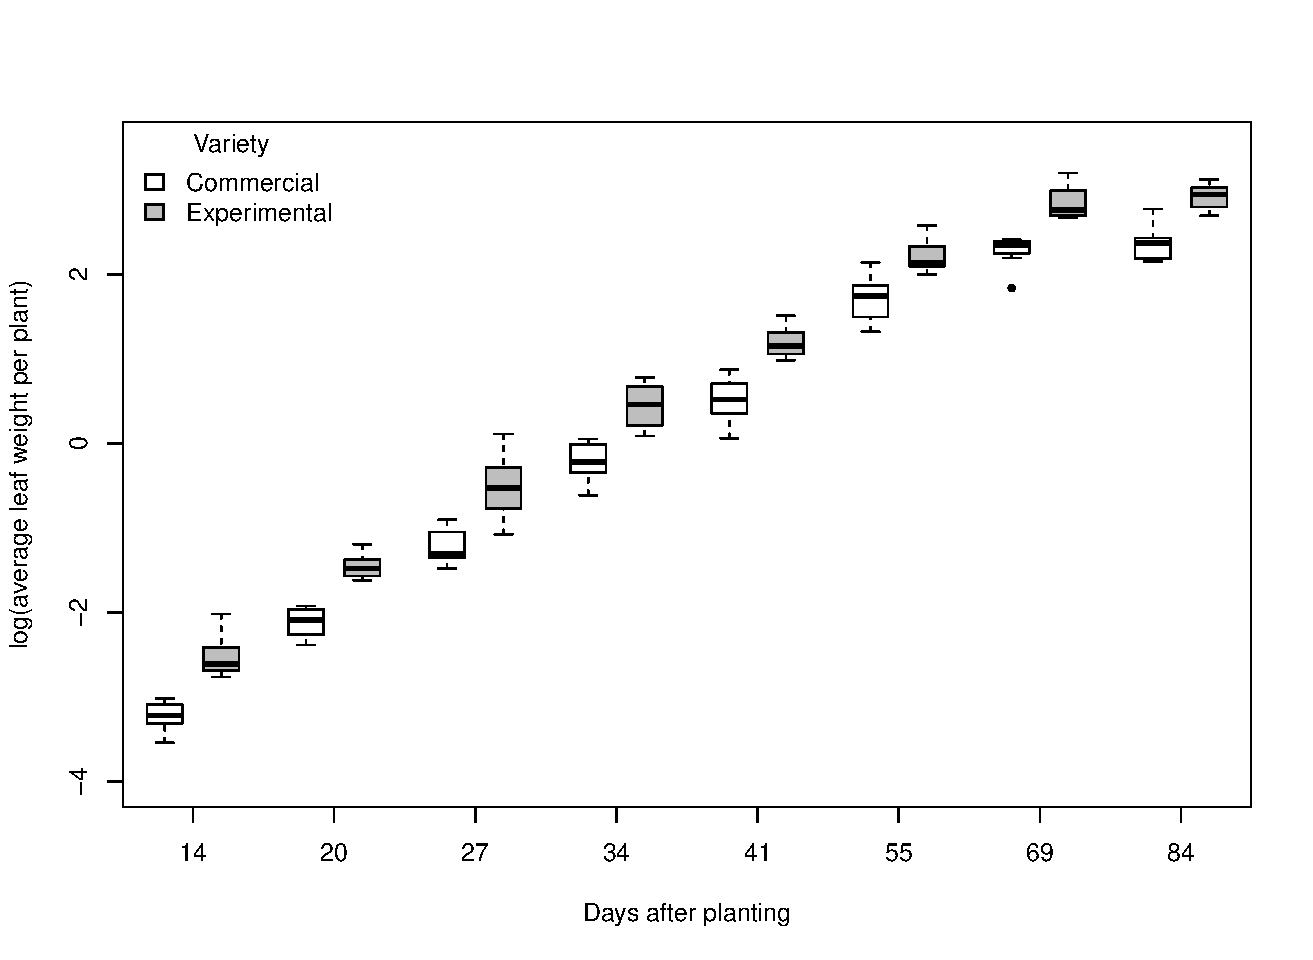
\includegraphics[width=\textwidth]{soybean}
\caption{Average leaf weight per plant over time.}
\label{sg}
\end{figure}

The data are analyzed using a model where the mean of the random variable $Y_{ij}$ ($j$th measurement of the average leaf weight per plant performed on the $i$th plot) is given by the following logistic-type curve:
$$\mu_{ij}=\dfrac{\beta_1+\beta_4\,\text{\tt Variety}_{ij}}{1+\exp\!\left(-(\text{\tt Time}_{ij}-\beta_2-\beta_5\,\,\text{\tt Variety}_{ij})/(\beta_3+\beta_6\,\text{\tt Variety}_{ij})\right)}, \quad i=1,\ldots,16;j=1,\ldots,8,$$
where ${\tt Variety}_{ij}=1$ if the soybean genotype is the experimental strain and ${\tt Variety}_{ij}=0$ otherwise. Therefore, the horizontal asymptote as $\text{\tt Time}\to \infty$ (also known as the carrying capacity), the inflection point and the scale parameter of $\mu$ for commercial varieties of soybean are $\beta_1$, $\beta_2$ and $\beta_3$; and $(\beta_1+\beta_4)$, $(\beta_2+\beta_5)$ and $(\beta_3+\beta_6)$ for experimental strains.

The starting value for $\bm{\beta}$ in the algorithm of parameter estimation is obtained through the built-in function {\tt SSlogis()}.
\begin{example}
> data(Soybean,package="nlme")
> Soybean2 <- subset(Soybean,Year=="1989")
> Soybean2 <- within(Soybean2,x <- ifelse(Variety=="P",1,0))
> 
> m0 <- gnmgee(weight ~ SSlogis(Time,b1,b2,b3), id=Plot, family=Gamma(identity), 
+              data=Soybean2)
> start <- c(coef(m0),rep(0,3))
> names(start) <- paste0("b",1:6)
> start
       b1        b2        b3        b4        b5        b6 
14.185637 51.453724  7.086697  0.000000  0.000000  0.000000 
\end{example}
Then, GEE models with quadratic variance function and different correlation matrix structures are fitted to the data.

\begin{example}
> m1 <- gnmgee(weight ~ (b1 + b4*x)/(1 + exp(-(Time - b2 - b5*x)/(b3 + b6*x))), 
+              start=start, id=Plot, family=Gamma(identity), data=Soybean2)
> m2 <- update(m1, corstr="Exchangeable")
> m3 <- update(m1, corstr="AR-M-dependent(1)")
> m4 <- update(m1, corstr="AR-M-dependent(2)")
> m5 <- update(m1, corstr="AR-M-dependent(3)")
> m6 <- update(m1, corstr="AR-M-dependent(4)")
\end{example}
As shown below, the correlation matrix structure chosen by the most of the criteria (that is, CIC, QIC, GHYC and PAC) is {\tt AR-M-dependent(3)}.

\begin{example}
> a <- CIC(m1, m2, m3, m4, m5, m6, verbose=FALSE)
> b <- QIC(m1, m2, m3, m4, m5, m6, verbose=FALSE)
> c <- GHYC(m1, m2, m3, m4, m5, m6, verbose=FALSE)
> d <- PAC(m1, m2, m3, m4, m5, m6, verbose=FALSE)
> e <- AGPC(m1, m2, m3, m4, m5, m6, verbose=FALSE)
> f <- SGPC(m1, m2, m3, m4, m5, m6, verbose=FALSE)
> cbind(a,QIC=b[,"QIC"],GHYC=c[,"GHYC"],PAC=d[,"PAC"],AGPC=e[,"AGPC"],SGPC=f[,"SGPC"])

  Object       Correlation   CIC      QIC  GHYC    PAC    AGPC    SGPC
1     m1      Independence 6.951 6163.648 8.126 0.9847 90.5844 95.2200
2     m2      Exchangeable 6.951 6163.648 7.552 0.9785 86.8152 92.2233
3     m3 AR-M-dependent(1) 6.795 6098.876 6.640 0.9753 86.1055 91.5136
4     m4 AR-M-dependent(2) 6.713 6095.808 6.622 0.9737 87.7812 93.9619
5     m5 AR-M-dependent(3) 6.708 6094.956 6.621 0.9736 89.7920 96.7453
6     m6 AR-M-dependent(4) 6.752 6115.573 6.673 0.9741 91.3912 99.1171
\end{example}
The chosen model is summarized as follows:

\begin{example}
> summary(m5)

Sample size
   Number of observations:  128
       Number of clusters:  16 
             Cluster size:  8 
*************************************************************
Model
        Variance function:  Gamma
            Link function:  identity
    Correlation structure:  AR-M-dependent(3)
*************************************************************
Coefficients
           Estimate Std.Error  z-value Pr(>|z|)
b1         10.58794   0.54866 19.29779  < 2e-16
b2         52.08512   0.99860 52.15828  < 2e-16
b3          7.01786   0.19565 35.87033  < 2e-16
b4          7.48960   0.88795  8.43475  < 2e-16
b5         -0.77453   1.29528 -0.59797  0.54986
b6          0.09913   0.24511  0.40441  0.68591
                                               
Dispersion  0.05686                            
*************************************************************
Working correlation
     [1]   [2]   [3]   [4]   [5]   [6]   [7]   [8] 
[1] 1.000 0.253 0.151 0.053 0.025 0.010 0.004 0.002
[2] 0.253 1.000 0.253 0.151 0.053 0.025 0.010 0.004
[3] 0.151 0.253 1.000 0.253 0.151 0.053 0.025 0.010
[4] 0.053 0.151 0.253 1.000 0.253 0.151 0.053 0.025
[5] 0.025 0.053 0.151 0.253 1.000 0.253 0.151 0.053
[6] 0.010 0.025 0.053 0.151 0.253 1.000 0.253 0.151
[7] 0.004 0.010 0.025 0.053 0.151 0.253 1.000 0.253
[8] 0.002 0.004 0.010 0.025 0.053 0.151 0.253 1.000
\end{example}
These results suggest that only the horizontal asymptote as $\text{\tt Time}\to \infty$ depends on the soybean variety. Their estimates are  $10.588$ grams and $18.078$ grams for commercial varieties and experimental soybean strains, respectively.



%\subsection{High-flow hemodialyzer}
%The dataset of this example, available in the {\tt hemodialyzer} object of {\tt glmtoolbox}, is composed of the columns {\tt Dialyzer}, {\tt TMP}, {\tt UFR} and {\tt Qb} (see Table~\ref{uh}). In vitro data on twenty high-flow hemodialyzers were analyzed by \cite{VC92} and \cite{V12}. High-flow dialyzers are used in hemodialysis to treat end-stage renal disease. The water transport kinetics of high-flow dialyzers are characterized by a functional relationship between the ultrafiltration rate ({\tt UFR} in liters/hour) at which water is removed and the transmembrane pressure ({\tt TMP} in mmHg) exerted on the dialyzer membrane at a fixed blood flow rate. The twenty dialyzers were evaluated in vitro using a single source of bovine blood at blood flow rates of 200 ({\tt Qb=``200''}) and 300 ({\tt Qb=``300''}) ml/min.

%The data are analyzed using a model where the mean of the random variable $Y_{ij}$ ($j$th measurement of the ultrafiltration rate performed on the $i$th high-flow dialyzer) is given by the following Gompertz-type curve:
%$$\mu_{ij}=(\beta_1+\beta_4\,\text{\tt Qb}_{ij})\exp\!\left(-(\beta_2+\beta_5\,\text{\tt Qb}_{ij})(\beta_3+\beta_6\,\text{\tt Qb}_{ij})^{\text{\tt TMP}_{ij}}\right),$$
%where ${\tt Qb}_{ij}=1$ if the blood flow rate is 300 ml/min and ${\tt Qb}_{ij}=0$ otherwise. Therefore, the expected ultrafiltration rate when the transmembrane pressure tends to be infinite is $\beta_1$ and $\beta_4$ for high-flow dialyzers at blood flow rates of 200 ml/min and 300 ml/min, respectively. In addition, the expected ultrafiltration rate when the transmembrane pressure tends to be $0$ is $\beta_1\exp(-\beta_2)$ and $(\beta_1+\beta_4)\exp(-(\beta_2+\beta_5))$ for high-flow dialyzers at blood flow rates of 200 ml/min and 300 ml/min, respectively.



\subsection{Amenorrhea rates over time}
The dataset of this example, available in the object {\tt amenorrhea} of {\tt glmtoolbox} and comprised of the columns named {\tt ID}, {\tt Dose}, {\tt Time}, and {\tt amenorrhea} (see Table~\ref{am}), arose from a longitudinal clinical trial of contracepting women \citep{MFBC88,FLW11}. A total of 1151 women completed menstrual diaries. The diary data were used to generate a binary sequence for each woman, indicating whether she had experienced amenorrhea (the absence of menstrual bleeding for a specified number of days) on the day of randomization and three additional 90-day intervals. This trial compared the two treatments (injections of 100 mg or 150 mg of depot-medroxyprogesterone acetate (DMPA)) in terms of how amenorrhea rates change over time with continued use of the contraceptive method. Figure \!~\ref{am1} shows that amenorrhea rates increase across treatments, but that it appears that women treated with 150 mg of DMPA are more likely to experience amenorrhea than those treated with 100 mg of DMPA at each time point. Moreover, Figure \!~\ref{am1} shows that the proportion of women experiencing amenorrhea (on the logit scale) increases non-linearly over time. A feature of this clinical trial is that there was substantial dropout. This is when a woman skips a particular injection and never returns for subsequent injections. Indeed, $38\%$ of the women dropped out before the trial ended; $17.2\%$ dropped out after receiving only one injection of DMPA, $13.5\%$ dropped out after receiving only two injections of DMPA, and $7.3\%$ dropped out after receiving three injections of DMPA. The subsequent statistical analysis is performed using the weighted GEE method, as it is assumed that the missing data pattern is better described by MAR than MCAR.

\begin{table}[!ht]
{\small
\begin{center}
\begin{tabular}{lll} 
 \hline
Column &  Role   &  Description\\ \hline
{\tt ID}  & Cluster/subject identifier & Identifier of the woman\\
{\tt Dose} & Explanatory variable & Treatment: ``100mg'' or ``150mg'' of DMPA\\
{\tt Time} & Explanatory variable & Number of 90-day intervals since the trial began\\
{\tt amenorrhea} & Response variable & 1 if experienced amenorrhea; 0 otherwise\\ 
 \hline
\end{tabular}
\end{center}
\caption{Columns in the object {\tt amenorrhea} of the package {\tt glmtoolbox}.}
\label{am}}
\end{table}

\begin{figure}[h!]
\centering
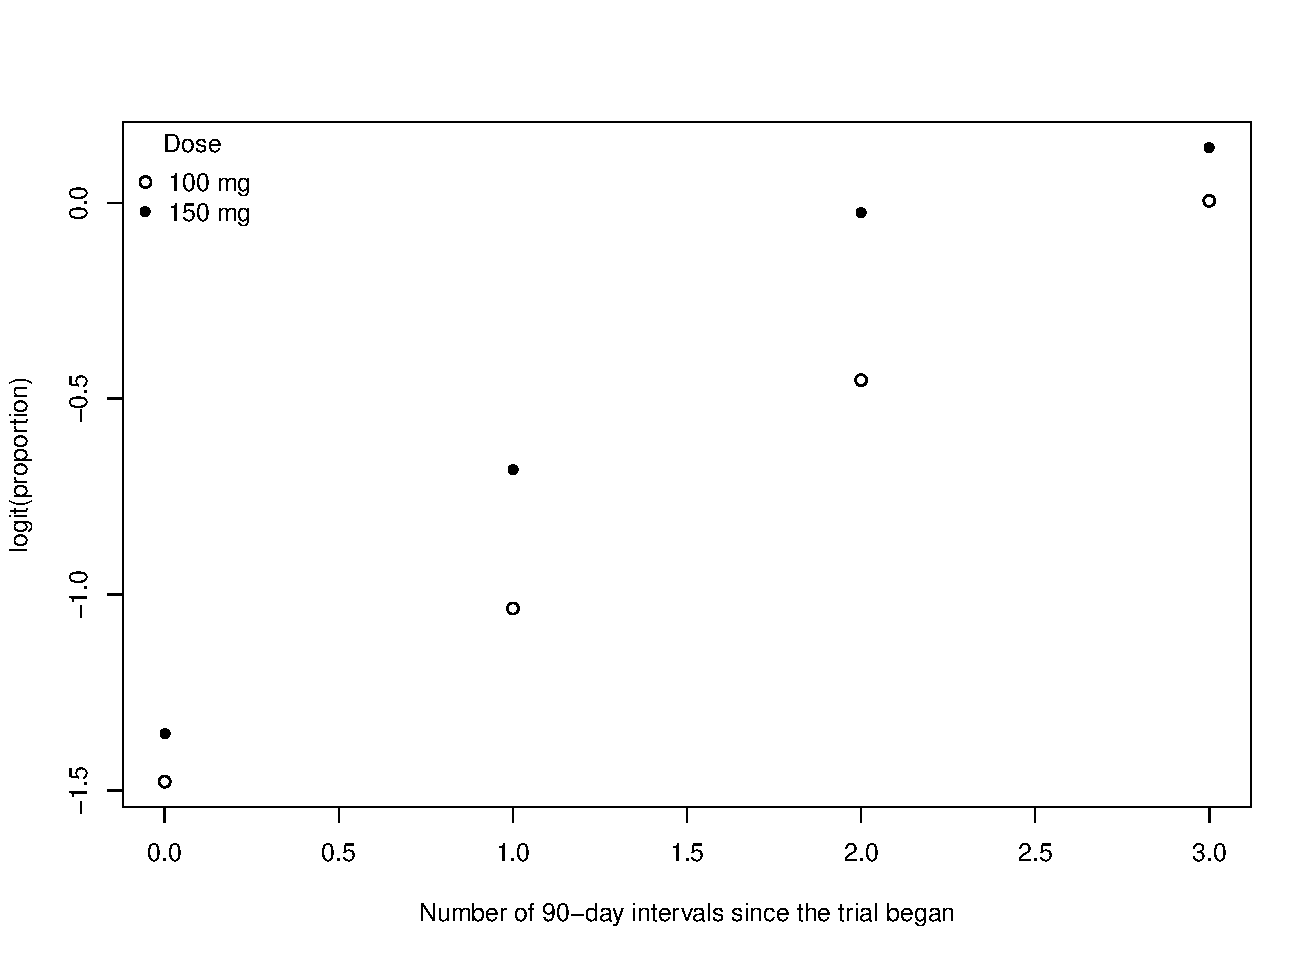
\includegraphics[width=\textwidth]{am}
\caption{Amenorrhea rates over time.}
\label{am1}
\end{figure}

%\begin{figure}[h!]
%\centering
%\psfrag{+}[][][0.65]{$\bullet$}
%\psfrag{-}[][][0.65]{$\circ$}
%\psfrag{e}[][][0.7]{\hspace{1cm}Dose}
%\psfrag{0}[][][0.65]{$0$}
%\psfrag{1}[][][0.65]{$1$}
%\psfrag{2}[][][0.65]{$2$}
%\psfrag{3}[][][0.65]{$3$}
%\psfrag{-1.5}[][][0.65]{$-1.5$}
%\psfrag{-1.0}[][][0.65]{$-1.0$}
%\psfrag{-0.5}[][][0.65]{$-0.5$}
%\psfrag{0.0}[][][0.65]{$0.0$}
%\psfrag{d}[][][0.65]{\hspace{1cm}150 mg}
%\psfrag{c}[][][0.65]{\hspace{1cm}100 mg}
%\psfrag{b}[][][0.8]{\hspace{-0.5cm}${\rm logit(proportion)}$}
%\psfrag{a}[][][0.8]{\hspace{-0.5cm}Number of 90-day intervals since the trial began}
%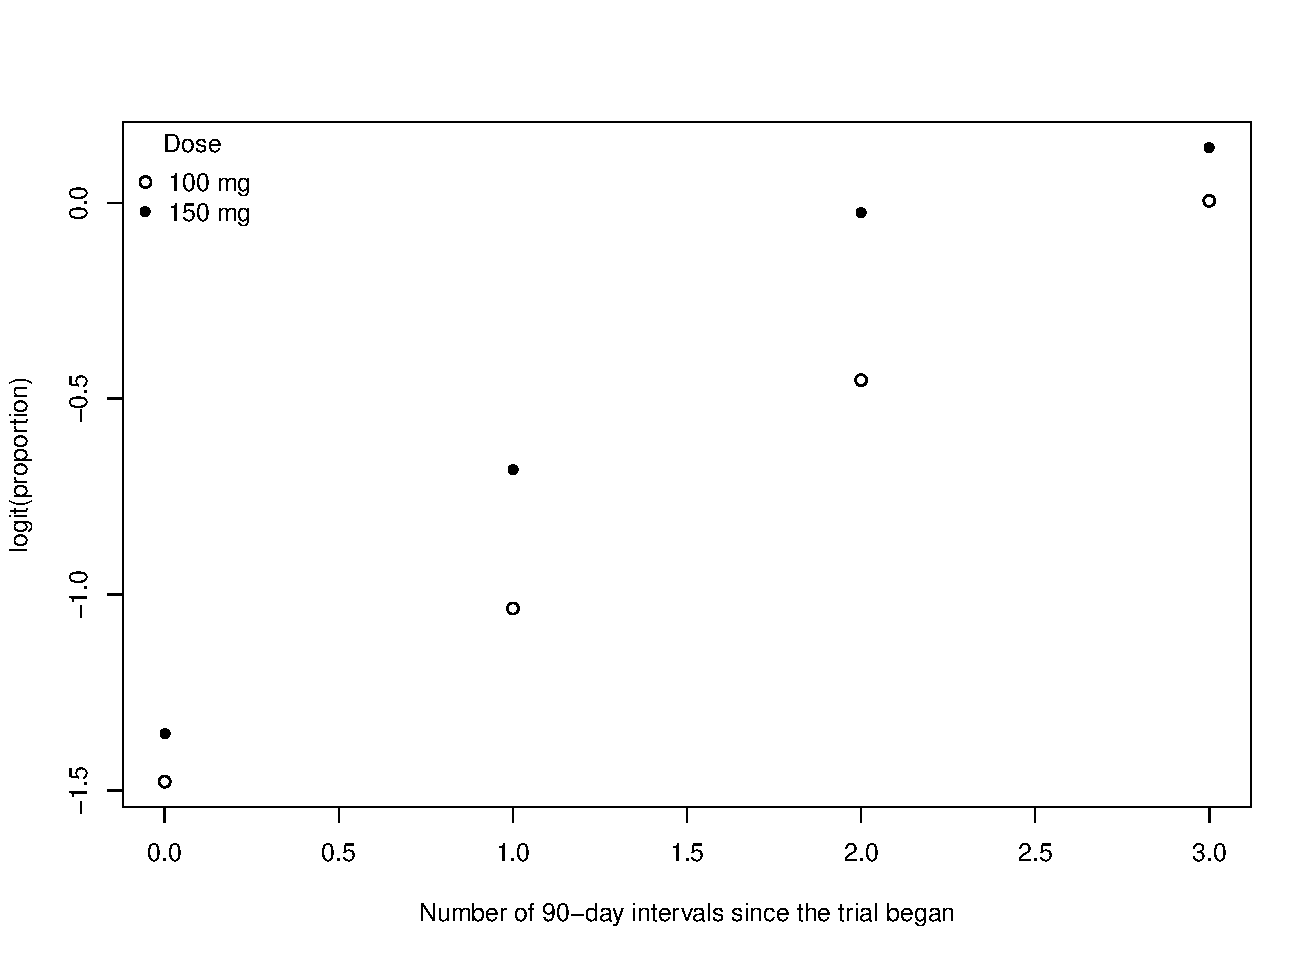
\includegraphics[width=\textwidth]{am}
%\caption{Amenorrhea rates over time.}
%\label{am1}
%\end{figure}

The data are analyzed using a model in which the probability of the $i$th woman experienced amenorrhea
at time $j$, denoted here by $\mu_{ij}$, is such that
$${\rm logit}(\mu_{ij})=1 + {\tt Time} + {\tt Time}^2 + {\tt Dose}.$$
For the missingness model the following systematic component is considered
$${\rm logit}(\pi_{ij})=1 + {\tt CTime} + {\tt Dose} + {\tt ylag1},$$
where {\tt CTime} is a categorical version of the explanatory variable {\tt Time} and {\tt ylag1} is defined to be $y_{i,j-1}$ if
$j>1$ and 0 if $j=1$. In addition, the structure of the working correlation matrix is set to be {\tt AR-M-dependent(1)}.
The observation-specified weighted GEE method results are the following:

\begin{example}
> data(amenorrhea)
> amenorrhea2 <- within(amenorrhea,{Ctime <- factor(Time)
+                                   Ctime <- relevel(Ctime,ref="1")
+                                   ylag1 <- c(0,amenorrhea[-length(ID)])
+                                   ylag1 <- ifelse(Time==0,0,ylag1)})
>
> fit1 <- wglmgee(amenorrhea ~ poly(Time,2) + Dose | Ctime + Dose + ylag1, 
+                 family=binomial, data=amenorrhea2, id=ID, corstr="AR-M-dependent(1)",
+                 scale.fix=TRUE, scale.value=1, level="observations")
> summary(fit1)

Clusters by dropout time
 Time 1    2    3    4   Freq   % 
   ---- ---- ---- ---- | ---- ----
      X    .    .    . |  198 17.2
      X    X    .    . |  155 13.5
      X    X    X    . |   84  7.3
      X    X    X    X |  714   62
   ---- ---- ---- ---- | ---- ----
                       | 1151  100
*************************************************************
Coefficients of missingness model
            Estimate Std.Error z-value  Pr(>|z|)    
(Intercept)   2.4349    0.1401 17.3845 < 2.2e-16 ***
Ctime1       -0.7247    0.1438 -5.0399 4.659e-07 ***
Ctime2       -0.5911    0.1469 -4.0250 5.698e-05 ***
Dose150mg    -0.0174    0.1049 -0.1663    0.8679    
ylag1        -0.5765    0.1122 -5.1369 2.793e-07 ***
*************************************************************
Observation-specific Weighted GEE

        Variance function:  binomial
            Link function:  logit
    Correlation structure:  AR-M-dependent(1)
*************************************************************
Coefficients
               Estimate Std.Error z-value Pr(>|z|)    
(Intercept)     -0.6835    0.0750 -9.1136  < 2e-16 ***
poly(Time, 2)1  40.7447    2.2598 18.0301  < 2e-16 ***
poly(Time, 2)2  -4.6883    1.9528 -2.4008  0.01636 *  
Dose150mg        0.2437    0.1061  2.2975  0.02159 *  
                                                      
Dispersion       1.0000                               
*************************************************************
Working correlation
     [1]   [2]   [3]   [4] 
[1] 1.000 0.414 0.171 0.071
[2] 0.414 1.000 0.414 0.171
[3] 0.171 0.414 1.000 0.414
[4] 0.071 0.171 0.414 1.000
\end{example}

According to the missingness model, the probability of remaining in the trial increases over time, regardless of the amenorrhea status reported by the women in the previous measurement. In addition, the missingness model indicates that the probability of remaining in the trial is higher for women without amenorrhea in their previous measurement, regardless of how many DMPA injections they have received. Therefore, the MAR assumption seems more appropriate than MCAR. Moreover, according to the model for $\mu$, the odds of experiencing amenorrhea is approximately $27.6\%=100\times[\exp(\hat{\beta}^{\rm Dose})-1]$ higher in women treated with 150 mg of DMPA than those treated with 100 mg of DMPA, where ${\beta}^{\rm Dose}$ represents the parameter associated with the explanatory variable {\tt Dose}. This is irrespective of the number of 90-day intervals since the experiment began. The results of the cluster-specific weighted GEE approach (do not show here) are very similar.

\section*{Acknowledgments}
The authors are grateful to the Editor and the referees for their helpful comments and suggestions that have led to significant improvements of this paper.


\hypertarget{refs}{}

\bibliography{RJreferences.bib}

\address{%
L.H. Vanegas\\
Departamento de Estadística, Universidad Nacional de Colombia\\%
Ciudad Universitaria, Bogotá\\ Colombia\\
%
%
%
\href{mailto:lhvanegasp@unal.edu.co}{\nolinkurl{lhvanegasp@unal.edu.co}}%
}

\address{%
L.M. Rondón\\
Departamento de Estadística, Universidad Nacional\\%
Ciudad Universitaria, Bogotá\\ Colombia\\
%
%
%
\href{mailto:lmrondonp@unal.edu.co}{\nolinkurl{lmrondonp@unal.edu.co}}%
}

\address{%
G.A. Paula\\
Instituto de Matemática e Estatística, Universidade de São Paulo\\%
Rua do Matão, 1010, São Paulo\\ Brazil\\
%
%
%
\href{mailto:giapaula@ime.usp.br}{\nolinkurl{giapaula@ime.usp.br}}%
}
